%%
%% Beginning of file 'sample62.tex'
%%
%% Modified 2018 January
%%
%% This is a sample manuscript marked up using the
%% AASTeX v6.2 LaTeX 2e macros.
%%
%% AASTeX is now based on Alexey Vikhlinin's emulateapj.cls 
%% (Copyright 2000-2015).  See the classfile for details.

%% AASTeX requires revtex4-1.cls (http://publish.aps.org/revtex4/) and
%% other external packages (latexsym, graphicx, amssymb, longtable, and epsf).
%% All of these external packages should already be present in the modern TeX 
%% distributions.  If not they can also be obtained at www.ctan.org.

%% The first piece of markup in an AASTeX v6.x document is the \documentclass
%% command. LaTeX will ignore any data that comes before this command. The 
%% documentclass can take an optional argument to modify the output style.
%% The command below calls the preprint style  which will produce a tightly 
%% typeset, one-column, single-spaced document.  It is the default and thus
%% does not need to be explicitly stated.
%%
%%
%% using aastex version 6.2
\documentclass[twocolumn]{aastex62}
\usepackage{amsmath}
%% The default is a single spaced, 10 point font, single spaced article.
%% There are 5 other style options available via an optional argument. They
%% can be envoked like this:
%%
%% \documentclass[argument]{aastex62}
%% 
%% where the layout options are:
%%
%%  twocolumn   : two text columns, 10 point font, single spaced article.
%%                This is the most compact and represent the final published
%%                derived PDF copy of the accepted manuscript from the publisher
%%  manuscript  : one text column, 12 point font, double spaced article.
%%  preprint    : one text column, 12 point font, single spaced article.  
%%  preprint2   : two text columns, 12 point font, single spaced article.
%%  modern      : a stylish, single text column, 12 point font, article with
%% 		  wider left and right margins. This uses the Daniel
%% 		  Foreman-Mackey and David Hogg design.
%%  RNAAS       : Preferred style for Research Notes which are by design 
%%                lacking an abstract and brief. DO NOT use \begin{abstract}
%%                and \end{abstract} with this style.
%%
%% Note that you can submit to the AAS Journals in any of these 6 styles.
%%
%% There are other optional arguments one can envoke to allow other stylistic
%% actions. The available options are:
%%
%%  astrosymb    : Loads Astrosymb font and define \astrocommands. 
%%  tighten      : Makes baselineskip slightly smaller, only works with 
%%                 the twocolumn substyle.
%%  times        : uses times font instead of the default
%%  linenumbers  : turn on lineno package.
%%  trackchanges : required to see the revision mark up and print its output
%%  longauthor   : Do not use the more compressed footnote style (default) for 
%%                 the author/collaboration/affiliations. Instead print all
%%                 affiliation information after each name. Creates a much
%%                 long author list but may be desirable for short author papers
%%
%% these can be used in any combination, e.g.
%%
%% \documentclass[twocolumn,linenumbers,trackchanges]{aastex62}
%%
%% AASTeX v6.* now includes \hyperref support. While we have built in specific
%% defaults into the classfile you can manually override them with the
%% \hypersetup command. For example,
%%
%%\hypersetup{linkcolor=red,citecolor=green,filecolor=cyan,urlcolor=magenta}
%%
%% will change the color of the internal links to red, the links to the
%% bibliography to green, the file links to cyan, and the external links to
%% magenta. Additional information on \hyperref options can be found here:
%% https://www.tug.org/applications/hyperref/manual.html#x1-40003
%%
%% If you want to create your own macros, you can do so
%% using \newcommand. Your macros should appear before
%% the \begin{document} command.
%%
\newcommand{\vdag}{(v)^\dagger}
\newcommand\aastex{AAS\TeX}
\newcommand\latex{La\TeX}

%% Reintroduced the \received and \accepted commands from AASTeX v5.2
%%\received{January 1, 2018}
%%\revised{January 7, 2018}
%%\accepted{\today}
%% Command to document which AAS Journal the manuscript was submitted to.
%% Adds "Submitted to " the arguement.
\submitjournal{ApJ}
%% Mark up commands to limit the number of authors on the front page.
%% Note that in AASTeX v6.2 a \collaboration call (see below) counts as
%% an author in this case.
%
%\AuthorCollaborationLimit=3
%
%% Will only show Schwarz, Muench and "the AAS Journals Data Scientist 
%% collaboration" on the front page of this example manuscript.
%%
%% Note that all of the author will be shown in the published article.
%% This feature is meant to be used prior to acceptance to make the
%% front end of a long author article more manageable. Please do not use
%% this functionality for manuscripts with less than 20 authors. Conversely,
%% please do use this when the number of authors exceeds 40.
%%
%% Use \allauthors at the manuscript end to show the full author list.
%% This command should only be used with \AuthorCollaborationLimit is used.

%% The following command can be used to set the latex table counters.  It
%% is needed in this document because it uses a mix of latex tabular and
%% AASTeX deluxetables.  In general it should not be needed.
%\setcounter{table}{1}

%%%%%%%%%%%%%%%%%%%%%%%%%%%%%%%%%%%%%%%%%%%%%%%%%%%%%%%%%%%%%%%%%%%%%%%%%%%%%%%%
%%
%% The following section outlines numerous optional output that
%% can be displayed in the front matter or as running meta-data.
%%
%% If you wish, you may supply running head information, although
%% this information may be modified by the editorial offices.
\shorttitle{p-Mode Oscillations in Highly Gravitationally Stratified Magnetic Solar Atmospheres}
\shortauthors{Griffiths et al.}
%%
%% You can add a light gray and diagonal water-mark to the first page 
%% with this command:
% \watermark{text}
%% where "text", e.g. DRAFT, is the text to appear.  If the text is 
%% long you can control the water-mark size with:
%  \setwatermarkfontsize{dimension}
%% where dimension is any recognized LaTeX dimension, e.g. pt, in, etc.
%%
%%%%%%%%%%%%%%%%%%%%%%%%%%%%%%%%%%%%%%%%%%%%%%%%%%%%%%%%%%%%%%%%%%%%%%%%%%%%%%%%

%% This is the end of the preamble.  Indicate the beginning of the
%% manuscript itself with \begin{document}.

\begin{document}

\title{p-Mode Oscillations in Highly Gravitationally Stratified Magnetic Solar Atmospheres}

%% LaTeX will automatically break titles if they run longer than
%% one line. However, you may use \\ to force a line break if
%% you desire. In v6.2 you can include a footnote in the title.

%% A significant change from earlier AASTEX versions is in the structure for 
%% calling author and affilations. The change was necessary to implement 
%% autoindexing of affilations which prior was a manual process that could 
%% easily be tedious in large author manuscripts.
%%
%% The \author command is the same as before except it now takes an optional
%% arguement which is the 16 digit ORCID. The syntax is:
%% \author[xxxx-xxxx-xxxx-xxxx]{Author Name}
%%
%% This will hyperlink the author name to the author's ORCID page. Note that
%% during compilation, LaTeX will do some limited checking of the format of
%% the ID to make sure it is valid.
%%
%% Use \affiliation for affiliation information. The old \affil is now aliased
%% to \affiliation. AASTeX v6.2 will automatically index these in the header.
%% When a duplicate is found its index will be the same as its previous entry.
%%
%% Note that \altaffilmark and \altaffiltext have been removed and thus 
%% can not be used to document secondary affiliations. If they are used latex
%% will issue a specific error message and quit. Please use multiple 
%% \affiliation calls for to document more than one affiliation.
%%
%% The new \altaffiliation can be used to indicate some secondary information
%% such as fellowships. This command produces a non-numeric footnote that is
%% set away from the numeric \affiliation footnotes.  NOTE that if an
%% \altaffiliation command is used it must come BEFORE the \affiliation call,
%% right after the \author command, in order to place the footnotes in
%% the proper location.
%%
%% Use \email to set provide email addresses. Each \email will appear on its
%% own line so you can put multiple email address in one \email call. A new
%% \correspondingauthor command is available in V6.2 to identify the
%% corresponding author of the manuscript. It is the author's responsibility
%% to make sure this name is also in the author list.
%%
%% While authors can be grouped inside the same \author and \affiliation
%% commands it is better to have a single author for each. This allows for
%% one to exploit all the new benefits and should make book-keeping easier.
%%
%% If done correctly the peer review system will be able to
%% automatically put the author and affiliation information from the manuscript
%% and save the corresponding author the trouble of entering it by hand.


%%\author[swat, cics]{M. K. Griffiths \corref{cor1}}
%%\author[acse]{V. Fedun}
%%\author[swat]{R. Erd\'{e}lyi}
%\author[cics]{D.Savas }
%\author{M.K.Griffiths\corref{cor1}\fnref{fn1},V.Fedun, D.Savas\tnoteref{tno2} and  R.Erd\'{e}lyi}
%\date{} % Activate to display a given date or no date (if empty),
         % otherwise the current date is printed 
%%\address[swat]{Solar Physics and Space Plasma Research Centre ($SP^{2}RC$), School of Mathematics and 
%%Statistics, University of Sheffield, Hicks Building, Hounsfield Road, S7 3RH, UK}
%%\address[cics]{Corporate Information and Computing Services, The University of Sheffield, 10-12 Brunswick Street, Sheffield, S10 2FN, UK}
%%\address[acse]{Department of Automatic Control and Systems Engineering, The University of Sheffield, Mappin Street, Sheffield, S1 3JD, UK}
%\fnref{<label(s)>}
%\tnotetext[<label>]{<title note text>}
%\cortext[cor1]{email: m.griffiths@sheffield.ac.uk}
%%\cortext[cor1]{Corresponding author at: Corporate Information and Computing Services, The University of Sheffield, 10-12 Brunswick Street, Sheffield, S10 2FN, UK. \linebreak e-mail address: m.griffiths@sheffield.ac.uk}




\correspondingauthor{M. Griffiths}
\email{m.griffiths@sheffield.ac.uk}

\author{M. Griffiths}
\affil{Research IT, The University of Sheffield, 10-12 Brunswick Street, Sheffield, S10 2FN, UK.}

\author{R. Erd\'{e}lyi}
\affiliation{Solar Physics and Space Plasma Research Centre ($SP^{2}RC$), School of Mathematics and Statistics, University of Sheffield, Hicks Building, Hounsfield Road, S7 3RH, UK}
%%\collaboration{(AAS Journals Data Scientists collaboration)}

\author{R. Zheng}
\affiliation{Shandong Provincial Key Laboratory of Optical Astronomy and Solar-Terrestrial Environment, and Institute of Space Sciences, Shandong University, Weihai 264209, China}
%\ead{r.zheng@sheffield.ac.uk}

\author{N. Gyenge}
\affil{Research IT, The University of Sheffield, 10-12 Brunswick Street, Sheffield, S10 2FN, UK.}

%% Note that the \and command from previous versions of AASTeX is now
%% depreciated in this version as it is no longer necessary. AASTeX 
%% automatically takes care of all commas and "and"s between authors names.

%% AASTeX 6.2 has the new \collaboration and \nocollaboration commands to
%% provide the collaboration status of a group of authors. These commands 
%% can be used either before or after the list of corresponding authors. The
%% argument for \collaboration is the collaboration identifier. Authors are
%% encouraged to surround collaboration identifiers with ()s. The 
%% \nocollaboration command takes no argument and exists to indicate that
%% the nearby authors are not part of surrounding collaborations.

%% Mark off the abstract in the ``abstract'' environment. 
\begin{abstract}

%The solar atmosphere exhibits a diverse range of wave phenomena one of the earliest to be discovered was the five minute oscillation, the p-mode. The analysis of wave propagation in the solar atmosphere may be used as a diagnostic tool to measure the physical characteristics of the suns atmospheric layers.

%{Aims.} 
With the objective of measuring the properties of the solar atmosphere and its magnetic structures we present a comparison of the analysis of results from observations and numerical simulations. The aim of the work reported in this paper is to gain understanding of the propagation characteristics of p-mode oscillations in the highly gravitationally stratified magnetic solar atmosphere.  
%\it{Methods.} 
The paper describes 3D numerical simulations of a model solar atmosphere employing simulation drivers resulting in oscillations mimicking the behaviour of  p-mode oscillations. MHD simulations used a model of the solar atmosphere constructed using the VALIIIc model \citet{Vernazza1981} of the quiet sun and including a uniform vertical cylindrically symmetric magnetic field. The simulations were run for different values of the magnitude of the magnetic field and a p-mode driver with a fixed period of 300s and corresponding to the well known 5 minute mode. This extended vertical velocity driver with a sinusoidal dependence and given wavelength was located at the photosphere. The magnetic field configuration of our model is a standing magnetic tube, passing through the chromosphere and the lower corona. Therefore, for the observational study we chose to  sample a typical active region.  Temporal analysis of the observational data for the region containing a small sunspot (solar pore), it was presumed that this features a similar magnetic structure as employed in our simulations. 

%\it{Results.} 
The paper reports the variation of the energy flux and oscillation frequency of the magnetosonic modes  and examines their variation with magnetic field strength. Comparison with observational data indicate the presence of oscillation signals with a frequency close to that measured for the simulated results. As well as demonstrating the propagation of energy into the solar corona a frequency shift of the simulated MHD wave modes is reported.

%\it{Conclusions.} 
We conclude that magnetic regions of the solar atmosphere are favourable regions for the propagation of energy by slow magnetosonic modes.  The results exhibit a  frequency shift,  for different values of the magnetic field. The obtained periodic behaviour is confirmed by observational data, featuring similar frequencies based on the intensity times series of SDO images.

%The result of an investigation of the dynamics and propagation of waves which are generated by the solar global eigenmodes. We present the results of a series of hydrodynamic simulations of a realistic model of the solar atmosphere. With the objective of recreating atmospheric motions generated by global resonant oscillation the simulations use a driver which is spatially structured and extended in a sinusoidal profile across the computational model. The drivers perturb the region at 0.5Mm above the bottom boundary of the model and coincident with the temperature minimum. A combination of the VALIIIC and McWhirter solar atmospheres and coronal density profiles were used as the background equilibrium model in the simulations. We present the results of a study of synthetic photospheric oscillations for a magnetic field free model of the quiet sun. To carry out the simulations, we employed the MHD code, SMAUG (Sheffield MHD Accelerated Using GPUs). Our results show that the amount of energy propagated into the solar atmosphere is consistent with a model of solar global oscillations described using the Klein-Gordon equation. 

%See the reference at the Astronomy Abstracts Service. SMAUG paper at ADS

%See the reference at the Astronomy Abstracts Service. SAC paper at ADS


%Each video shows the value of the vertical component of the plasma velocity (z-component) along different slices through the simulation box. The scale shows the velocity value in m/s. The green vectors show the velocity directions along a single slice through the simulation. The green surface at a height of 3.5Mm is the 2MK temperature isosurface. The simulation box is 4Mmx4Mm along the base and the height of the box is 5.7Mm. The driver for the simulations is located at a height of 0.5Mm.


%Each video is labelled using 3 numbers. The first number is the driver period in seconds. The following 2 integers are each of the mode indices for the x and y direction respectively.


%Our results show that the amount of energy propagated into the solar atmosphere is consistent with a model of solar global oscillations described using the Klein-Gordon equation. 



\end{abstract}

%% Keywords should appear after the \end{abstract} command. 
%% See the online documentation for the full list of available subject
%% keywords and the rules for their use.
\keywords{editorials, notices --- 
miscellaneous --- catalogs --- surveys}

%% From the front matter, we move on to the body of the paper.
%% Sections are demarcated by \section and \subsection, respectively.
%% Observe the use of the LaTeX \label
%% command after the \subsection to give a symbolic KEY to the
%% subsection for cross-referencing in a \ref command.
%% You can use LaTeX's \ref and \label commands to keep track of
%% cross-references to sections, equations, tables, and figures.
%% That way, if you change the order of any elements, LaTeX will
%% automatically renumber them.
%%
%% We recommend that authors also use the natbib \citep
%% and \citet commands to identify citations.  The citations are
%% tied to the reference list via symbolic KEYs. The KEY corresponds
%% to the KEY in the \bibitem in the reference list below. 

\section{Introduction} \label{sec:intro}

Observational, theoretical and computational studies of the sun reveal a diversity of  structures and complex dynamics. This is clearly revealed by imagery from solar telescopes. The culmination of studies of the dynamics of the coronal loop structures  in the solar atmosphere and in the solar chromosphere has developed our understanding of the range of different magnetic field structures. %The images from SDO in nine AIA passbands (\ref{sdoaia}) display some of these structures such as active regions, coronal holes and quiet regions.
Despite our armoury of observations and diverse range of computational models it still remains a challenge to make sense of this complex menagerie of dynamical structures, understand solar coronal heating and more generally space weather phenomena. Development of our understanding requires computational models enabling us to study the relationship between structures in the solar atmosphere and the continual dynamical processes.

%% \begin{figure}[h]\label{sdoaia}
%% 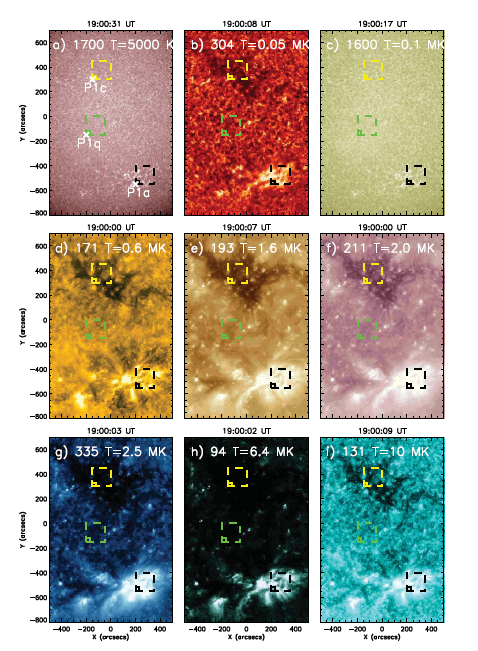
\includegraphics[scale=1.0]{imrescale/sdo_aia-img.png}
%% \caption{Activity in the solar corona and IR in nine AIA passbands on 22 August 2010 during solar minimum.
%% The dashed boxes outline the typical regions of the Sun,  Active Region (AR) , Quiet Sun (QS), and Coronal Hole (CH) on each panel.}
%\caption{Initial Magnetic Field Configuration, radial field distribution, uniform in the vertical direction with a maximum value of 100G }
%% \end{figure}

An example of the dynamical complexity are the ubiquitous five minute oscillations in the solar atmosphere, these are referred to as the solar global acoustic oscillations or p-modes. They are interpreted as trapped acoustic waves, i.e. standing acoustic oscillations. The solar p-modes perturb the photosphere, the main restoring force for these acoustic oscillations is pressure.  Earlier models had assumed reflection at the photosphere, and at most allowed evanescence above the photosphere. There is now increasing evidence for leakage of these modes. The p-modes were seen as resonant modes between the steep change in density at the solar surface and trapped beneath by the increase of the sound speed causing refraction and eventually forming a lower turning point in the interior. The observation of the resulting standing modes are now widely used as a diagnostic tool to understand the physical characteristics of the solar layers.

The complexity and variety of magnetic structures in the solar atmosphere gives rise to a complex mixture of waves providing powerful diagnostics to aid our understanding and advance our knowledge. The characteristics of generated waves is dependent on the motions at the footpoints of magnetic field concentrations and includes those in the intergranular lanes. For example vortical motions have been demonstrated to generate alfvenic waves \citet{Fedun2011}. 

In this paper we report on the results of numerical simulations of photospheric p-mode oscillations in a model solar atmosphere with a uniform and vertical magnetic field. First, we consider the variety of magnetic structures in the solar atmosphere and review the wave motions which are observed in these regions. This is followed with a description of the solar atmospheric model, magnetic field configuration and the simulation method we used to model p-mode oscillations in a model magnetic solar atmosphere.

\section{Structures in the Solar Atmosphere } \label{sec:structures}
The highly dynamical solar Chromosphere exhibits many different kinds of structures. For example faculae, pores or the bright areas near to and around sunspots. Pores are smaller counterparts of sunspots upto a few Mm across. The faculae are bright spots forming in the trenches between solar granules, they constantly form and dissipate over time scales of several minutes and they are formed near magnetic field concentrations.   The bright areas which extend away from active regions in the active network are called plage regions, these regions of the magnetic chromosphere are referred to as the network. The magnetic fields in this area diffuse away into the quiet sun regions. The magnetic network is a network of lines which outline super granules, these are convective regions about 30Mm across, they possess strong horizontal flows. The motions within the super granules result in the concentration of bundles of magnetic field lines.  The mean photospheric field in the internetwork region is 100-300G.  Solar active regions contain sunspots which have sizes between 1Mm and 50Mm. Active regions producing flares may have fields which easily exceed the normal range of 100-500G. As well as these massive concentrations, solar magnetograms reveal many north poles in the quiet photosphere, this is known as the magnetic carpet. These structures can be observed in figure \ref{magneticnetwork}. Along with the coronal funnels arising from grain boundaries, the picture shows a range of network loops with temperatures which can be in the range $10^{5}$K to $10^{6}$K.

%\begin{figure}[h]\label{solarmagneticnetwork}
%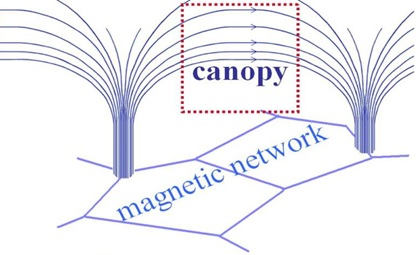
\includegraphics[scale=1.0]{imrescale/solar-magnetic-network.jpg}
%\caption{The Solar Magnetic Network.}
%%\caption{Initial Magnetic Field Configuration, radial field distribution, uniform in the vertical direction with a maximum value of 100G }
%\end{figure}

\begin{figure}[h]\label{magneticnetwork}
\centering
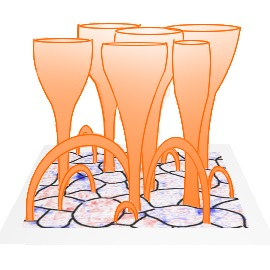
\includegraphics[scale=1.0]{imrescale/solar-network-v1.jpg}
\caption{The Solar Magnetic Network.}
%\caption{Initial Magnetic Field Configuration, radial field distribution, uniform in the vertical direction with a maximum value of 100G }
\end{figure}

 
The dynamical phenomena of concern in this paper result from waves and oscillations in the solar atmosphere. The upward propagation of waves through the solar atmosphere can result in coronal heating, frequency shifts and other wave phenomena. A range of wave transformations may occur including reflection and refraction by atmospheric structures. Our initial studies were relevant for the quiet inter-network region of the non magnetic solar chromosphere, which is similar to the quiet sun with magnetic fluxes in the range 5-10G. These are the regions between the magnetic flux concentrations. The coronal holes are cold regions of plasma  and  have open field lines allowing solar particles to escape, during the solar minima these regions can cause space weather disturbances. 

Given this variety of solar regions it is recognised that the modes of oscillation with periods of 3 and 5 minutes behave in different ways in the solar atmosphere network, inter network, plage and faculae regions. What is striking is the varied behaviour for different magnetic structures and the influence of reflecting layers such as the transition layer influencing upward and downward propagation.  The power spectra presented in figure 1 of \citet{Griffiths2018} exhibit a variation of propagation characteristics at different levels within the solar atmosphere and within different regions such as coronal holes, the quiet sun and active regions. In general the power spectra indicate a preponderance of long period 5 minute waves with frequencies in the range 1.5-5mHz. Also observed are the distinctive peaks for the short period 3 minute waves (with frequencies in the range 5-8mHz). The power spectra exhibit peaks in much longer period ranges for example 12 minute waves  (frequencies in the range 1.1-1.5mHz)  and 16 minute waves (frequencies 1-1.1mHz). For the quiet sun regions the 5 minute modes are stronger at photospheric levels and diminished higher up in the corona, but note a small peak for the AIA 211 corresponding to 2.0MK. 

%\begin{figure}[h]\label{powerspectra}
%\includegraphics[scale=0.5]{imrescale/powerspectra.jpg}
%\caption{Power spectra}
%%\caption{Initial Magnetic Field Configuration, radial field distribution, uniform in the vertical direction with a maximum value of 100G }
%\end{figure}

The review of \citet{Khomenko2013} summarises this complex picture. For the network and inter network regions the short period 3 minute modes propagate from the photosphere to the chromosphere only in restricted areas of the network cell interiors. The longer 5 minute modes propagate efficiently to the chromosphere in the close proximity of the magnetic network elements. These long-period network halos are most prominent in the photosphere, but are also present in the chromosphere; and are observed to be co-spatial with chromospheric “magnetic shadows” for 3 min waves. The plage and faculae regions possess more complex magnetic structures and exhibit a more complex pattern.  Observations show that the power of the 5 minute modes increase significantly in the chromosphere. For the short period  3 minute modes there is an enhancement, both in the photosphere and in the chromosphere. These power enhancements are known as “halos” and have been widely reported \cite{Kontogiannis2010}. 

\section{Motivation} \label{sec:motivation}

Given the complexity of the dynamics and the diversity of structures in the solar atmosphere. It is understood that a truly realistic model is challenging requiring a hybrid multi-disciplined approach. In order to develop a model providing a representation of the solar atmosphere it is necessary to establish that the modelling tools give a consistent behaviour in idealised test cases and that there is a consistency between the computational and theoretical models. Many computational MHD simulations of the sun have been undertaken some of the approaches have resulted in an encouraging degree of realism  \citet{Vogler2005}, \citet{Gudiksen2011}. Computational MHD simulations of the propagation of waves in 3D solar atmospheres was undertaken by \citet{Fedun2009}. Initially they considered hydrodynamical models, in later simulations \citet{Fedun2011} \citet{Vigeesh2012} reported results for magnetized solar atmospheres featuring an idealized flux tube. These models with point drivers demonstrated the leakage of magneto-acosustic energy into the solar atmosphere. The work of \citet{Khomenko2013} and  \citet{Santamaria2015} reviewed and presented 2D computational MHD modelling of wave propagation in magentic features such as sunpots and arcades. Such models reveal that energy reaches the corona along vertical magnetic fields. Although magentic energy is concentrated below the transition evidence was presented for conversion of Acoustic energy to fast magnetic modes.

Our initial models were hydrodynamic simulations of a realistically stratified model of the solar atmosphere representing its lower region from the photosphere to low corona \citet{Griffiths2018}. The objective was to model atmospheric perturbations, propagating from the photosphere into the chromosphere, transition region and low corona. The perturbations caused by the photospheric global oscillations were represented in the simulations using photospheric drivers to mimic the solar p-modes. These hydrodynamic modelling studies demonstrated that the energy flux predictions were in agreement with the results of the two layer Klein-Gordon model supporting our interpretation of the interaction of solar global oscillations with the solar atmosphere.

The simulations also revealed a consistency between the frequency-dependence of the energy flux in the numerical simulations and power flux measurements obtained from SDO and demonstrated the propagation of energy into the mid- to upper-atmosphere of the quiet Sun, this occured for a range of frequencies and may explain observed intensity oscillations for periods greater than the well known 3-minute and 5-minute oscillations. It was also found that energy flux propagation into the lower solar corona is strongly dependent on the particular wave modes. 

In this paper we present results for 3D numerical MHD simulations with an extended driver representing photospheric p-mode oscillations in a magnetic solar atmosphere, the objective is to gain understanding of the propagation characteristics of the p-mode oscillations. 

\section{Numerical Computation Methods}

The 3D numerical simulations described here were undertaken using Sheffield MHD Accelerated Using GPUs \citep[SMAUG,][]{Griffiths2015}, the GPU implementation of the Sheffield Advanced Code \citep[SAC,][]{Shelyag2008}. SAC and SMAUG are numerical MHD solvers allowing us to model the time-dependent evolution of photospheric oscillations in the solar atmosphere. SAC is a derivative of the versatile advection code (VAC) developed by \citep{Toth1996}.  The general system of ideal MHD equations are
\begin{eqnarray}
&& {{\partial \rho}\over{\partial t}}+\nabla\cdot\left( \rho{\mathbf v}\right)=0, \label{e1} \\
&& {{\partial ( \rho {\bf v})}\over{\partial t}}+\nabla\cdot\left( {\bf v}\rho {\bf v}-{\bf B B}\right)+\nabla p_t=\rho{\bf g}, \label{e2}\\
&& \frac{\partial e}{\partial t}+\nabla\cdot\left({\bf v}e-{\bf B B}\cdot{\bf v}+{\bf v}p_{t}\right)+\nabla p_t=\rho{\bf g}\cdot{\bf v}, \label{e3} \\
&& {{\partial{\bf B}}\over{\partial t}} +\nabla \cdot\left(  {\bf vB}-{\bf Bv}\right)=0. \label{e4}
\end{eqnarray}
Here, $\rho$ is the mass density, $\mathbf v$ is the velocity,  $\mathbf B$ is the magnetic field, $\it{e}$ is the energy density, $p_{t}$ is the total pressure and $\mathbf g$ is the gravitational acceleration vector.
The total pressure $p_{t}$ is written as
\begin{equation}
p_{t}=p_{k}+{{\bf B}^{2}\over{2}}, \label{e5}
\end{equation}
where $p_k$ is the kinetic pressure given by
\begin{equation}
p_{k}=\left(\gamma -1\right)\left(e-\frac{\rho {\mathbf v}^{2}}{2}-\frac{{\mathbf B}^{2}}{2}\right). \label{e6}
\end{equation}
Equations (\ref{e1}) - (\ref{e6}) are applicable to an ideal compressible plasma. The SAC code is based on perturbed versions of these equations, thus the variables $\rho $, $e$ and  $\mathbf B$ are expressed in terms of perturbed and background quantities as
\begin{eqnarray}
&& \rho = \tilde{\rho}+\rho_b, \nonumber \\
&& e = \tilde{e}+e_b,  \nonumber \\
&& {\mathbf B} = \tilde{\mathbf B}+{\mathbf B}_b.  \nonumber 
\end{eqnarray}
where $\tilde{\rho}$ is the  perturbed density,  $\tilde{e}$ is the perturbed energy and $\tilde{\bf B}$  is the perturbed magnetic field. The background quantities with a subscript $\it{b}$ do not change in time, as we assume a magneto-hydrostatic equilibrium of the background plasma. 

The SMAUG code is a fully non-linear MHD numerical finite element solver for simulating, linear and non-linear wave propagation in strongly magnetised plasma with structuring and stratification. The solver applies a fourth order central differencing technique to the spatial derivatives and the Euler or fourth order Runge-Kutta method to solve the temporal derivatives. By virtue of their symmetry, central differencing schemes are conservative, with the desired side effect that the solver conserves the divergence of the magnetic field. The application of central differencing to hyperbolic differential equations results in unstable solutions with a spurious oscillatory behaviour.

Hyper-diffusion and hyper-resistivity are implemented to achieve numerical stability of the computed solution of the MHD equations \citep[see for example][]{Caunt2001}. The primary purpose of the diffusion terms is to compensate for the anti-diffusion from truncation errors arising in the computation of temporal and spatial derivatives. When the diffusion is correctly tuned the resulting evolution is non-diffusive. In addition, the diffusion terms control the steepness of shocks by becoming large wherever the compression is large. The full set of MHD equations, including the hyper-diffusion source terms are given in \citet{Griffiths2015} and \citet{Shelyag2008}.

\begin{figure}[h]\label{inimagfieldplot}
\centering
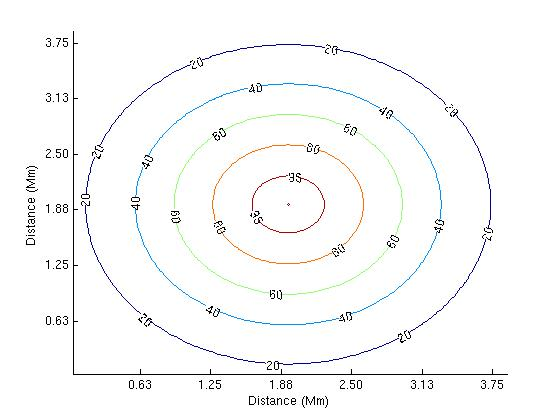
\includegraphics[scale=0.475]{imrescale/bfield100G.jpg}
\caption{Initial Magnetic Field Configuration, radial field distribution, uniform in the vertical direction with a maximum value of 100G }
\end{figure}

\break

\section{Computational Model}
%%CORRECT DESCRIPTION OF MAGNETIC FIELD CONFIGURATION NEEDED AN MHS ATMOSPHERE
%%With the magnetic-field-free quiet Sun in mind, we set $\vec{B}=0$ in the MHD equations.  
The computational box used for our simulations represents a volume of the solar atmosphere  with dimensions $L_{ x}= 4$ Mm and $L_{y} =4$ Mm. The model utilises a representation of the solar atmosphere with gravitational stratification in the $z$-direction and with a height of $L_{z} =6$ Mm. The computational box comprises an array of elements of dimension $128 \times128 \times128$. The upper boundary of our model  is in the solar corona and the lower boundary in the photosphere. The SMAUG code is well suited for modelling the leakage of wave energy from the photosphere, through the transition region and into the corona. We used open boundary conditions for all of the boundaries, allowing the modelling of wave propagation for time scales characterised by the 5-minute $p$-mode induced oscillations. The computational model is excited by an extended vertical velocity driver located at the photosphere, this acoustic $p$-mode driver excites waves which propagate into a realistic 3D model of the solar atmosphere. In the following two sections we describe the solar atmospheric model and the implementation of the driver. 

For the hydrodynamical studies reported in  \citet{Griffiths2018}, simulation drivers were used which behave like p-mode oscillations with varying modes and periods. We performed MHD simulations using our model of the solar atmosphere and including a uniform vertical cylindrically symmetric magnetic field. Simulations were run for different values of the magnitude of the magnetic field. For all of the simulations a p-mode driver was used with period 300s and mode (2,2). The 300s driver  was used as this corresponds to the well known 5 minute mode. The (2,2) mode was used because our earlier study demonstrated its effectiveness with energy propagation.


%following figures are shown in \citet{Griffiths2018}(figure 2)
%\section{Magnetohydrostatic Solar Atmospheric Model}
%To simulate oscillatory phenomena in the solar corona a physically representative model of the solar atmosphere is needed. 
%\begin{figure}[h]
%\begin{center}
%\mbox{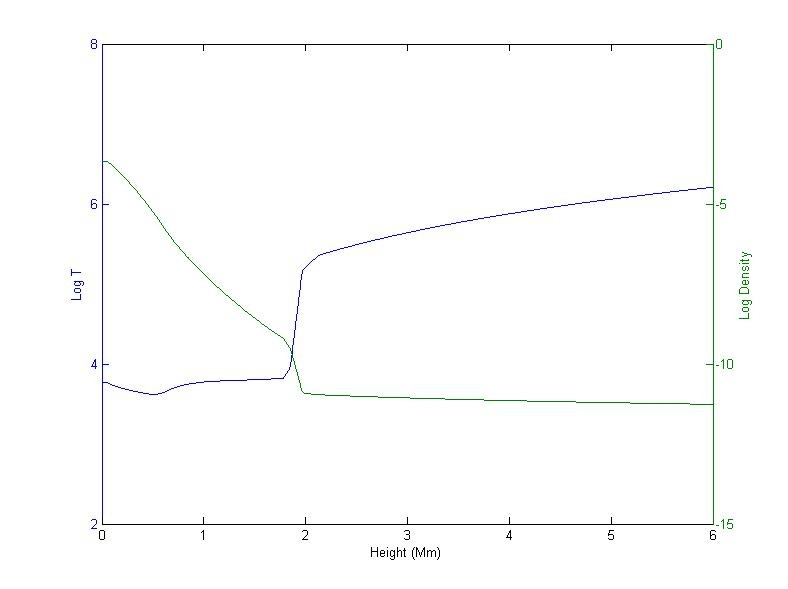
\includegraphics[scale=1.8]{imrescale/VAL3C_rho_temp_fig1L.jpg}}  
%\mbox{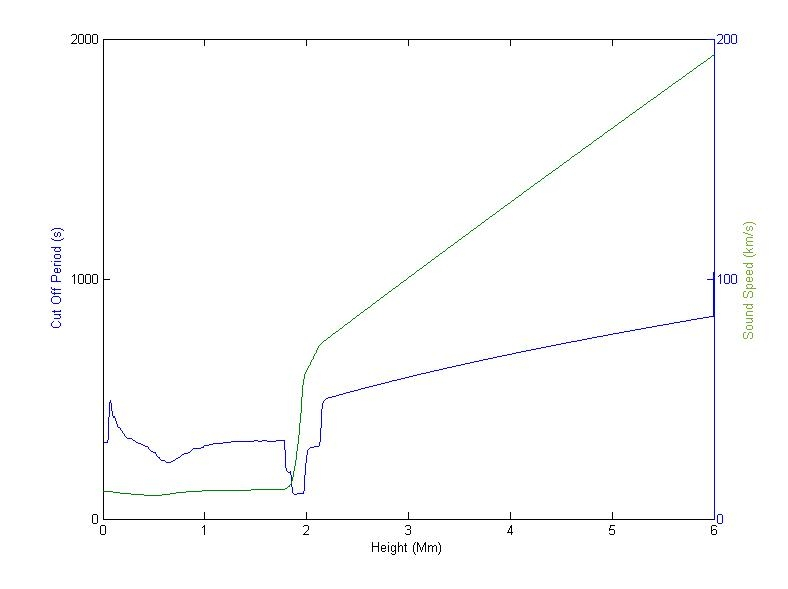
\includegraphics[scale=1.8]{imrescale/soundspeedVAL3C_profile_fig1R.jpg}}
%\par
%\end{center}
%\caption{Temperature and density profiles (left) used for the model atmosphere and cut-off frequency at different heights (right).}
%\label{Fig1}
%\end{figure}


The model atmosphere employed here is an observationally derived semi-empirical representation of the quiet sun. With the fundamental assumption of hydrostatic equilibrium a model of the chromosphere in equilibrium is constructed using the VALIIIc model, see \citet{Vernazza1981}. For the region of the solar atmosphere above 2.5 Mm the results of the energy balance model of solar coronal heating has been used \citep[see][]{McWhirter1975}, his model includes an acoustic contribution comparable to the hydrostatic pressure. An option is the use of a parametrisation of the temperature of the solar atmosphere which may be a smoothed step function profile see \citet{Murawski2010}. Results have demonstrated the need for observationally derived semi-empirical models of the solar atmosphere. There is much discussion about model validity and the work undertaken to 
demonstrate the reliability of the assumptions used to construct realistic models of the solar chromosphere, see \citet{Carlsson1995}, \citet{Kalkofen2012}. The contention arises from the dynamical nature of the solar chromosphere; for example local dynamo action has been suggested as a mechanism of Joule heating in the solar chromosphere, see \citet{Leenaarts2011}.  

A hydrostatic model for the solar atmosphere can be constructed by making use of the ideal gas equation for the solar atmosphere.
\begin{equation}
p_{0}=\frac{\rho_{0}R_{gas}T_{0}}{\mu}  , \label{e8}
\end{equation}

$R_{gas}$ is the gas constant and $\mu$ is mean atomic weight. For the fully ionized higher region of the atmosphere $\mu=0.5$, whilst lower down we set $\mu=1$. $p_{0}$, $\rho_{0}$ and $T_{0}$ are the pressure, density and temperature distributions for the stratified solar atmosphere. The scale height for the atmosphere is
\begin{equation}
H(z)=\frac{R_{gas}T_{0}(z)}{g}  , \label{e10}
\end{equation}

By using the scale height with the temperature profile from the VALIIIc and McWhirter model, the pressure equation is integrated over the atmospheric height and the density profile was computed.
\begin{equation}
\frac{dp_{0}(z)}{dz}=-\rho_{0}g   , \label{e9}
\end{equation}

Illustrations of the resulting temperature and density profiles can be seen in Figure 2 of \citet{Griffiths2018}. For the simulations described here we use a simplistic model which is uniform in the vertical (z) direction the field is cylindrical using the parametrisation in equation \ref{e7}. For the simulations here the effective cylinder radius is fixed at $R=0.5Mm$, simulations were run for different values of $B_{max}$.




\begin{equation}
B_{z}=B_{max} e^{-\frac{x^2+y^2}{R^2}} , \label{e7}
\end{equation}
Where $R=0.25Mm$
Magnetic field model for solar atmosphere. Since the field is uniform in the vertical direction the model atmosphere in hydrostatic equilibrium is in magnetohydrostatic equilibrium.

\begin{figure*}\label{vzplot_bv0g_76_150_225}
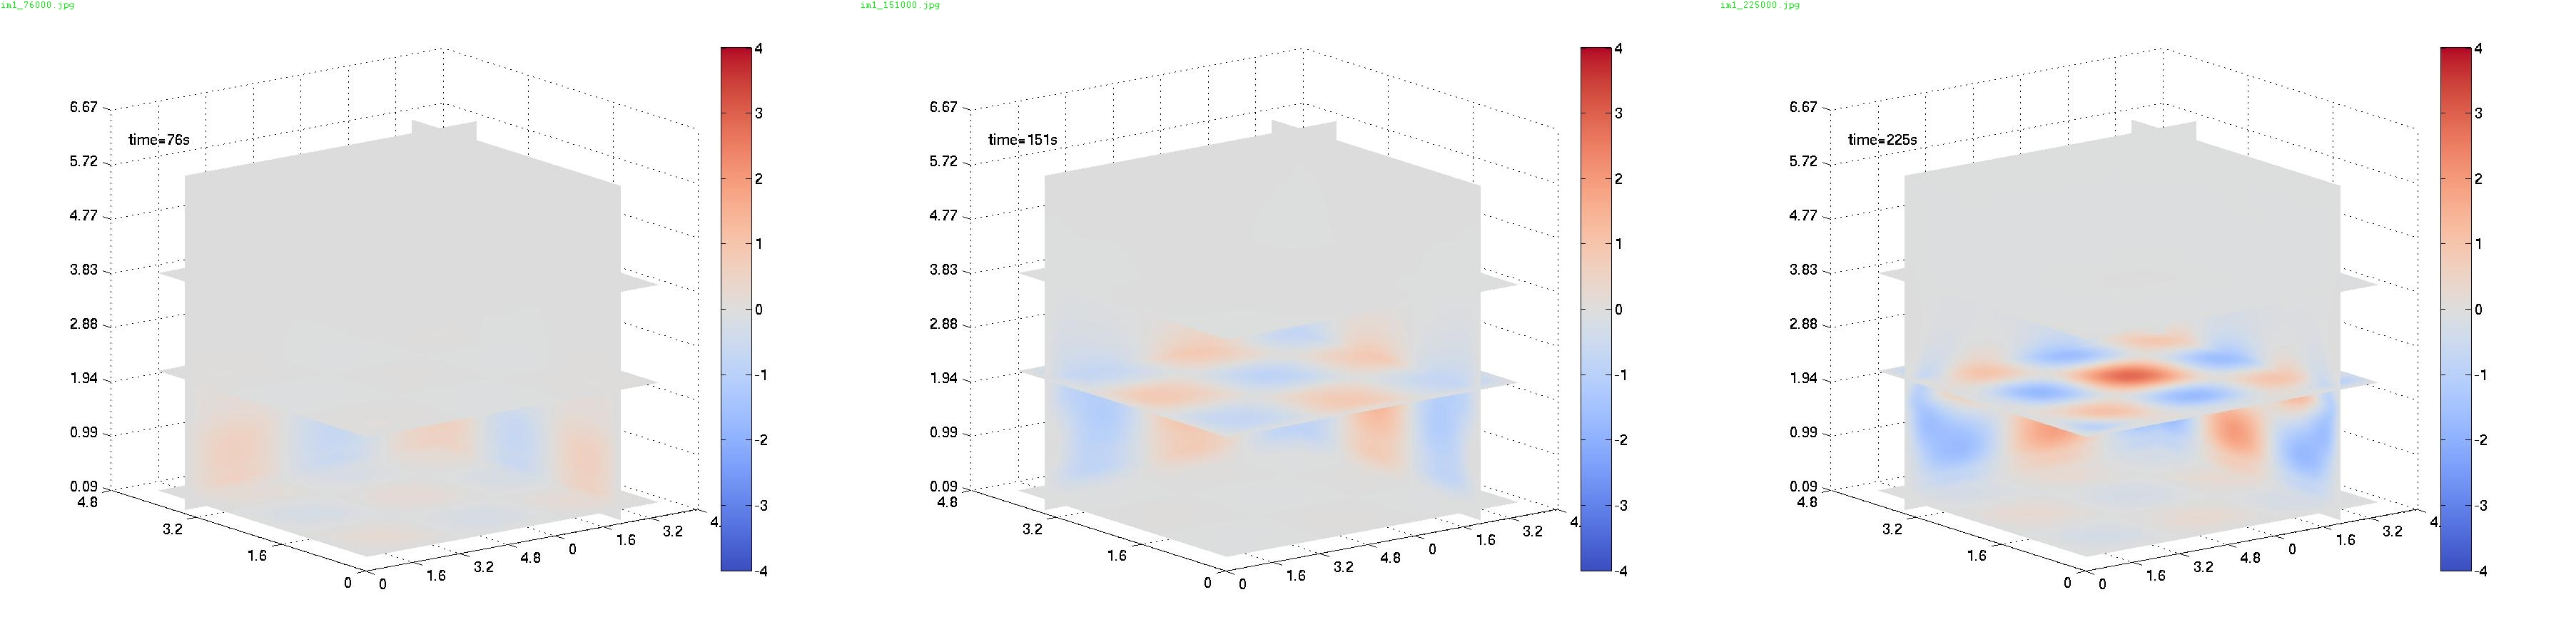
\includegraphics[scale=0.146]{imrescale/vz_bv0g_76_150_225.jpg}
\caption{Vertical Component of the Velocity for Different Sections of the Simulation for 76s, 150s and 225s for a field free configuration.}
\end{figure*}

\begin{figure*}\label{vzplot_bv50g_76_150_225}
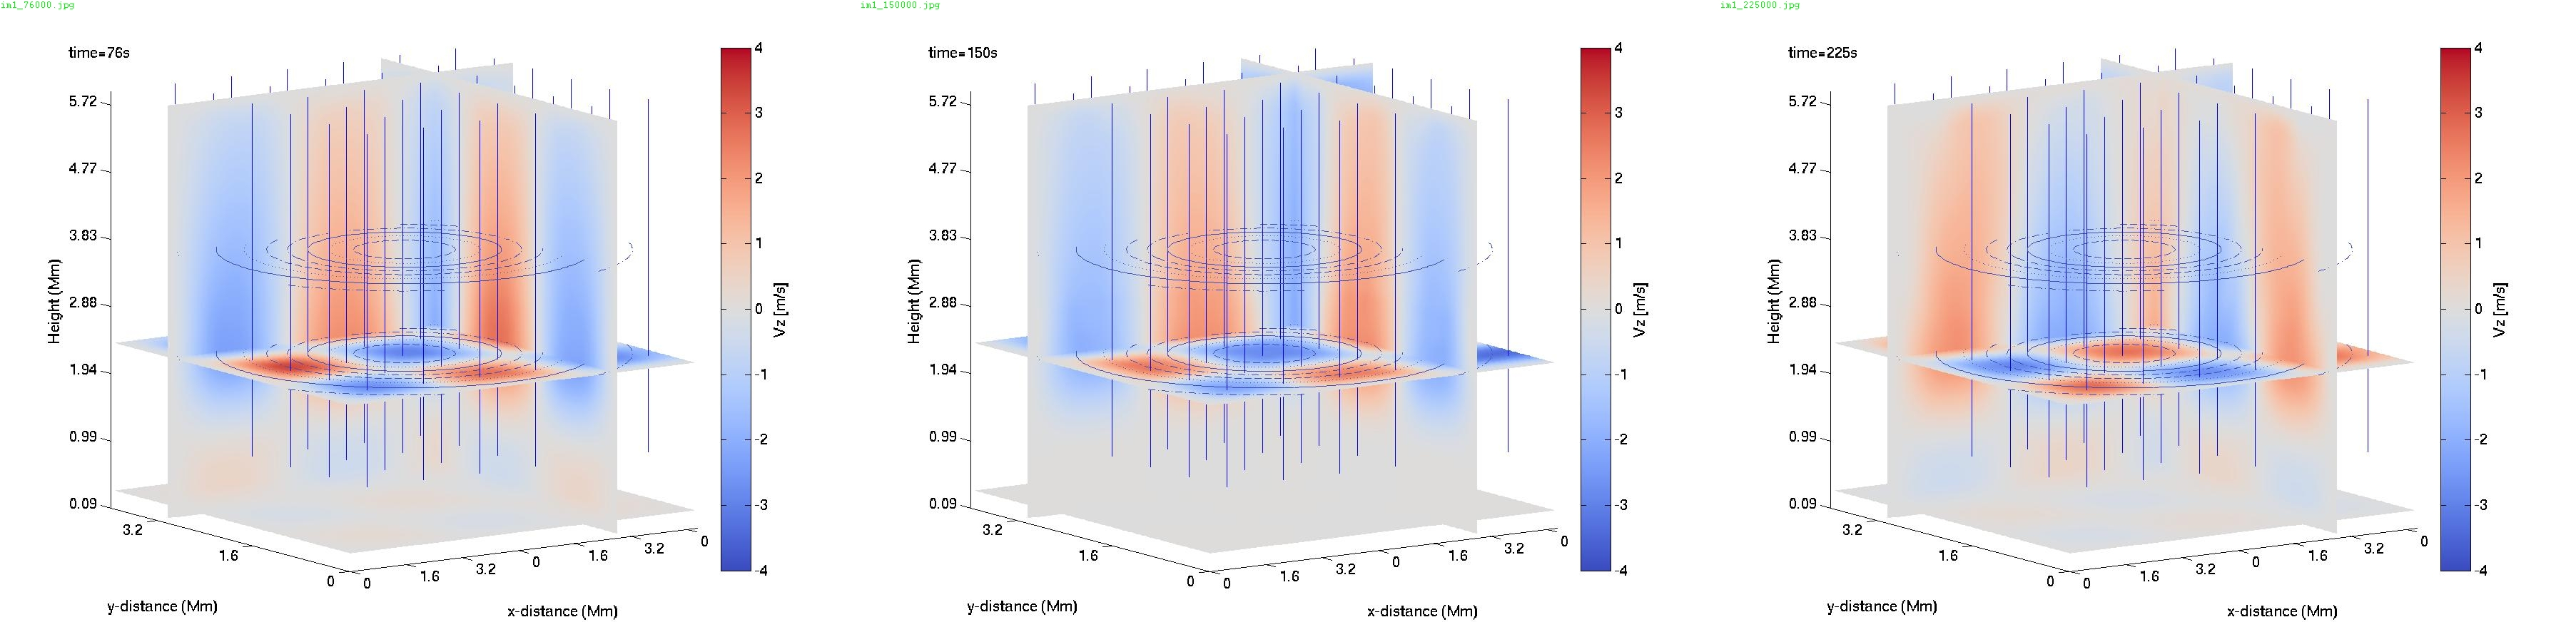
\includegraphics[scale=0.146]{imrescale/vz_bv50g_76_150_225.jpg}
\caption{Vertical Component of the Velocity for Different Sections of the Simulation for 76s, 150s and 225s for a vertical field with maximum field of 50G}
\end{figure*}

\begin{figure*}\label{vzplot_bv75g_76_150_225}
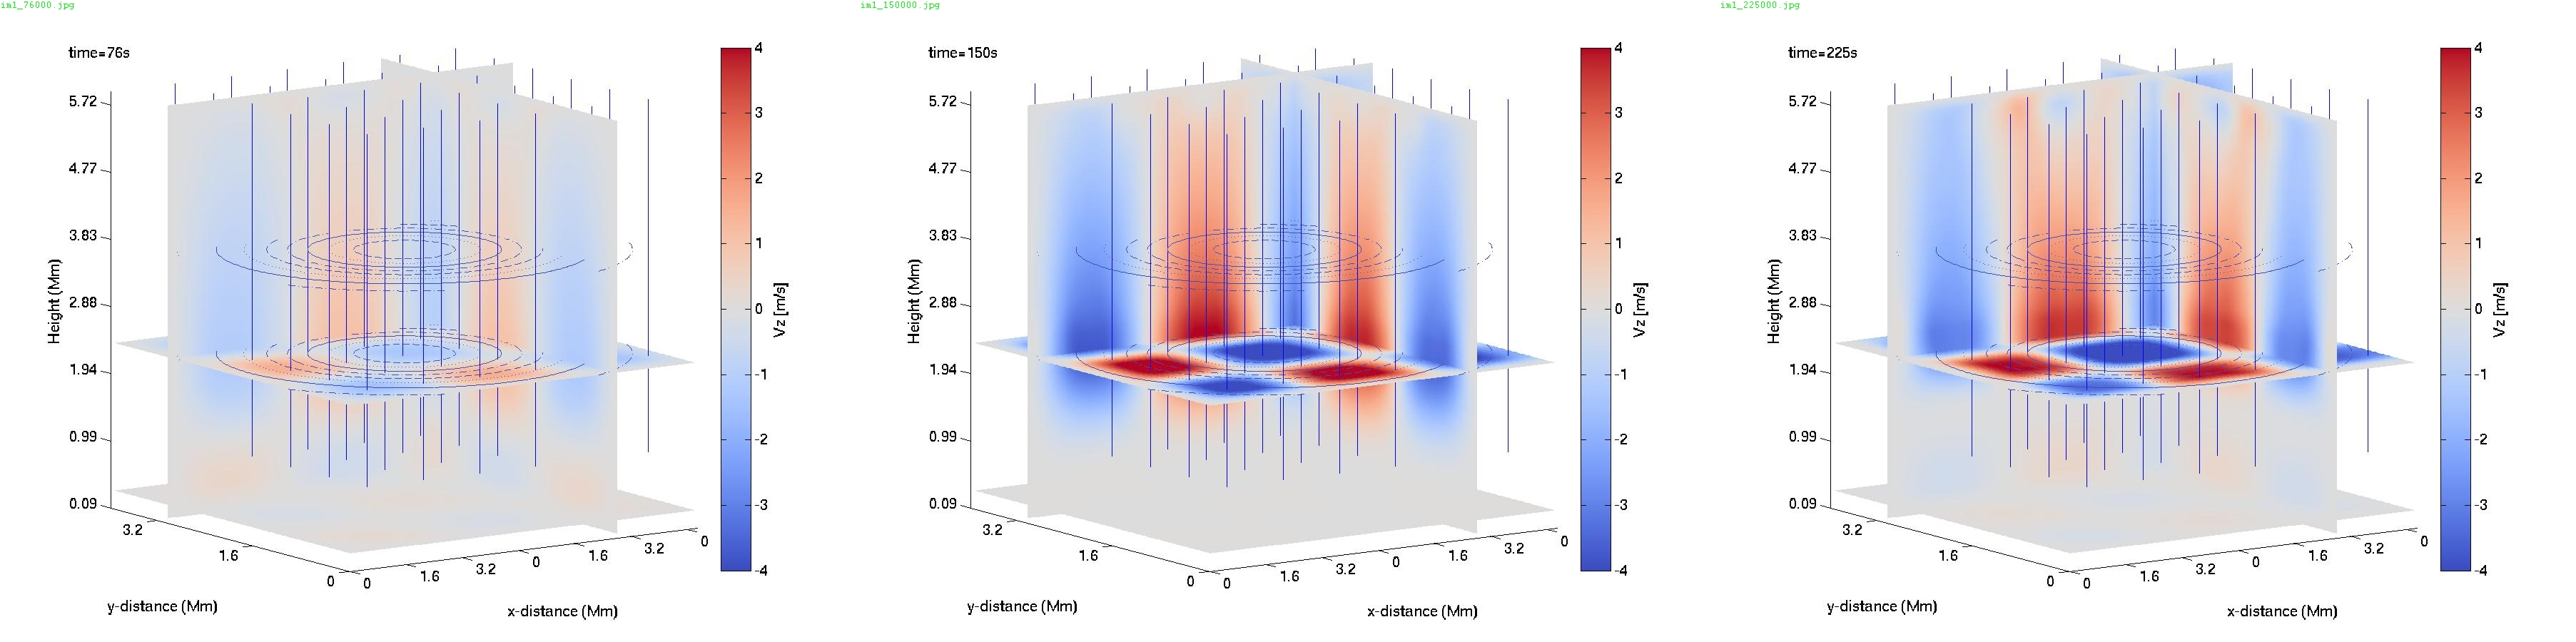
\includegraphics[scale=0.146]{imrescale/vz_bv75g_76_150_225.jpg}
\caption{Vertical Component of the Velocity for Different Sections of the Simulation for 76s, 150s and 225s for a vertical field with maximum field of 75G}
\end{figure*}

\section{Numerical Drivers for $p$-mode Oscillations}
 The overview of observational studies identified a range of physical phenomena resulting in oscillatory behaviour and delivering energy into the solar atmosphere.  Using drivers characterising the solar global oscillations, we extend the earlier work undertaken by  \citet{Malins2007A}, for their study, point drivers were used to represent periodic buffeting of turbulent motions in the photosphere. The results of the study demonstrated surface waves and structures in the transition region and highlighted the characteristics of the oscillatory phenomena as a result of frequency cut-offs induced by the stratified solar atmosphere. For the simulations presented in this paper, the whole boundary of the model was perturbed.  In the real Sun, photospheric $p$-mode oscillations have a horizontal wavelength and coherence. For the simulations reported here, the excitations are represented with a vertical velocity driver located at the photosphere. This acoustic $p$-mode driver excites waves which propagate 
into a realistic 3D model of the solar atmosphere. Simulations were run with drivers representing different modes. For example,  an extended driver with a sinusoidal dependence and a wavelength of 8 Mm applied along the 
middle of the base of a computational domain of dimension 4 Mm represents  a {\it fundamental mode}. 
A driver with wavelength 4 Mm applied the same way represents the {\it first harmonic} and {\it second harmonic} 
with wavelength 2 Mm was also considered. Drivers may be constructed as an ensemble of these solar 
global eigenmodes.  The driver is represented by the expression shown in equation (\ref{e8}) 


\begin{align}
V_{z} & =A_{nm} \sin\left(\frac{2\pi t}{T_s} \right)\sin\left(  \frac{(n+1)\pi x}{L_x} \right) \nonumber \\
&\sin\left(\frac{(m+1)\pi y}{L_y} \right) \exp\left( -\frac{(z-z_0)^2}{\Delta z^2} \right),
\label{e8}
\end{align}


\begin{figure*}\label{vzplot_bv100g_76_150_225}
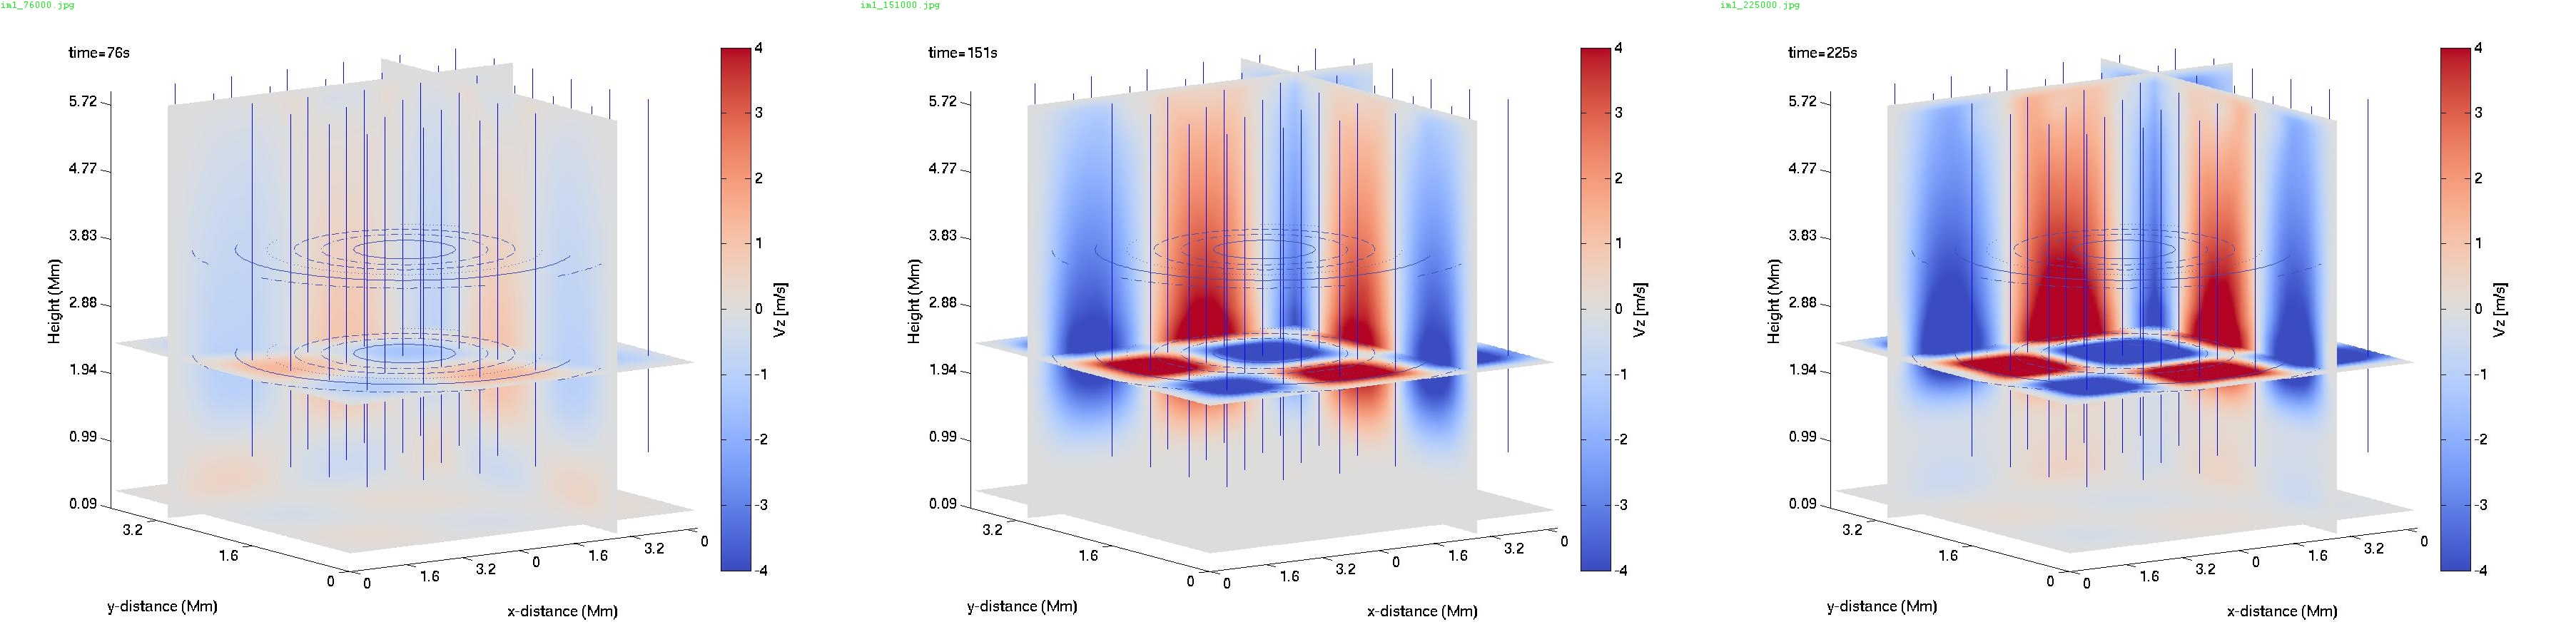
\includegraphics[scale=0.146]{imrescale/vz_bv100g_76_150_225.jpg}
\caption{Vertical Component of the Velocity for Different Sections of the Simulation for 76s, 150s and 225s for a vertical field with maximum field of 100G.}
%\caption{Initial Magnetic Field Configuration, radial field distribution, uniform in the vertical direction with a maximum value of 100G }
\end{figure*}



In equation (\ref{e8}) $L_{x}$ and $L_{y}$ are the lengths of the base of the simulation box in the $x$ and $y$ directions respectively. $T_{s}$ is the period and $A_{nm}$ is the amplitude of the driver, the indices $n$ and $m$ define the mode. $\Delta z$ is the width of the driver which was set here to $4km$, the parameter $z_{0}$ was set so that the vertical driver location is coincident with the location of the temperature minimum which is 0.5 Mm above the lower boundary of the model i.e. the photosphere.   Since we are investigating the leakage of energy into the solar atmosphere, it is necessary to ensure that for the different modes the driver amplitude is set to a value so that the same total amount of energy is delivered over the model cross section and per unit time.  The simulations presented use the parameter $A_{nm}$=500\, ms$^{-1}$ with the mode indices set to $n,m=2$. 




\section{Magnetoacoustic Waves in Uniform Vertical Magnetic Field Configurations}
Magnetohydrodynamic simulations have been performed with p-mode oscillations of the photospheric layer and for magnetic field strengths of 0G, 50G, 75G and 100G. The plasma $\beta$ for the model decreases rapidly from a value of 12 at the lower boundary of the simulation domain, $\beta$ decrease to 1 at 0.5Mm. From the top of the transition layer to the upper boundary of the model $\beta $ has a constant value of $1\times 10^{-6}$. It is anticipated that for the region with $\beta \approx 1$, mode conversion occurs with full or partial conversion to magnetohydrodynamic modes. 

\ref{vzplot_bv0g_76_150_225}, \ref{vzplot_bv50g_76_150_225}, \ref{vzplot_bv75g_76_150_225} and \ref{vzplot_bv100g_76_150_225} show the vertical component of the velocity at various times for different sections through the simulation box. Each figure corresponds to a vertical field configuration with field strength 0G, 50G, 75G and 100G respectively. There is a clear difference between the purely hydrodynamic, 0G case and the MHD cases. The figures exhibit evidence of a fast moving magneto-acoustic wave mode. These figures compare the wave modes at a quarter, half and three-quarters of a cycle. The propagation speed is consistent with that of a fast magneto-acoustic mode. Even a small magnetic field appears to enhance the motion of plasma in the corona and  there is an apparent difference in phase between the magnetic field cases. As well as an increase in the velocity amplitude with increasing magnetic field there is a small shift in the frequency of the oscillation. This observation is consistent with the theoretical prediction of \citet{Hindman1996} who predicted shifts in the microhertz and nanohertz range for fields between $1kG$ and$50G$. 

The full set of videos for all the simulations performed have been made available on the digital media repository hosted by The University of Sheffield, see \citet{Griffiths2018}. Each video shows the value of the vertical component of the plasma velocity ($z$-component) along different slices through the simulation box. The scale shows the velocity in m/s.  Each video is labelled using the magnetic field strength in Gauss.






%Figure \ref{dt_vvert_5b2_2_2Mm_1Mm_0p5MM_0G_25G_50G_100G_line} 
%Figure \ref{dt_vvert_100G_300s_180s}

Figure \ref{dt-5b2_2_100G-midchrom} shows a plot of the z component of the velocity at different times for a location at the centre of the box. Different curves are plotted for different heights. The red, green and blue curves correspond to a height  of 0.5Mm, 1Mm and 2Mm respectively. Although the periods are the same as that of the driver there are different shifts for different heights the shift corresponds to the propagation time for that height. The velocities for the magnetic field cases are larger than for the field free case.

%Time distance plots for the model with the 100G field are shown in figure  \ref{dt_vvert_100G_300s_180s_1p4Mm} these plots show %the case of the driver period of 300s and 180s. 

% figure \ref{dt_vvert_100G_300s_180s}
The wavespeeds computed from distance-time plots for the 300s period driver are shown in table \ref{Tablewavespeeds_300s} speeds for the 0G field are consistent with the speed of sound in the solar atmosphere whilst the speeds for the non zero magnetic field are consistent with propagation speeds for magnetosonic modes. 
\begin{table}\label{wavespeeds}
\centering
\begin{tabular}{c c c c c}
\hline
Wave Speed (km/s)   &  0G  &  50G &  75G & 100G\\
\hline
2Mm & 12.6  &   96.5       &   47.7      &  25.2     \\
\hline
1Mm & 10.1  &    64.1      &   44.4     &   45.4      \\
\hline
0.5Mm & 8.7  &   45.4      &   37.8      &   32.3    \\
\hline

\end{tabular} 
\caption{The table shows wave speeds obtained from the distance-time plots for the 300s period driver with magnetic fields of 0G,50G, 75G and 100G.}
\label{Tablewavespeeds_300s}
\end{table}

\begin{table*}\label{energyflux}
\centering
\begin{tabular}{c c c c c}
\hline
Magnetic Field (G)   &  1Mm  &  2Mm &  4Mm & 5.5Mm \\
\hline
0G & 0.2625  &    0.0021      &   1.4846 x $10^{-6}$     &   1.7399 x $10^{-6}$      \\
\hline
50G & 0.5401  &   -4.9441       &   0.882      &  0.5417     \\
\hline
75G & 0.1978  &    -1.576 x $10^{-4}$      &   1.1586 x $10^{-6}$     &   8.1936 x $10^{-7}$      \\
\hline
100G & 0.0165  &   -1.8664      &   0.7116      &   0.4092    \\
\hline

\end{tabular} 
\caption{The table shows the time averaged and integrated energy flux ratio obtained  for the 300s period driver with magnetic fields of 0G,50G, 75G and 100G.}
\label{energyfluxratio}
\end{table*}


\ref{vxplot_bv0g_76_150_225}, \ref{vxplot_bv50g_76_150_225}, \ref{vxplot_bv75g_76_150_225} and \ref{vxplot_bv100g_76_150_225} show the horizontal component of the velocity at various times for different sections through the simulation box. Each figure corresponds to a vertical field configuration with field strength 0G, 50G, 75G and 100G respectively. In the lower region there is evidence of slow magnetoacoustic wave propagation perpendicular to the field lines. Since the source terms perturb only the vertical component of the velocity and the model is cylindrically symmetric, pure Alfvenic modes are not expected. 








%PLOTCHANGE OF VELOCITY -Z WITH TIME AT DIFFERENT SECTIONS



%\begin{figure}[h]\label{vz_0G_50G_75G_100G_76}
%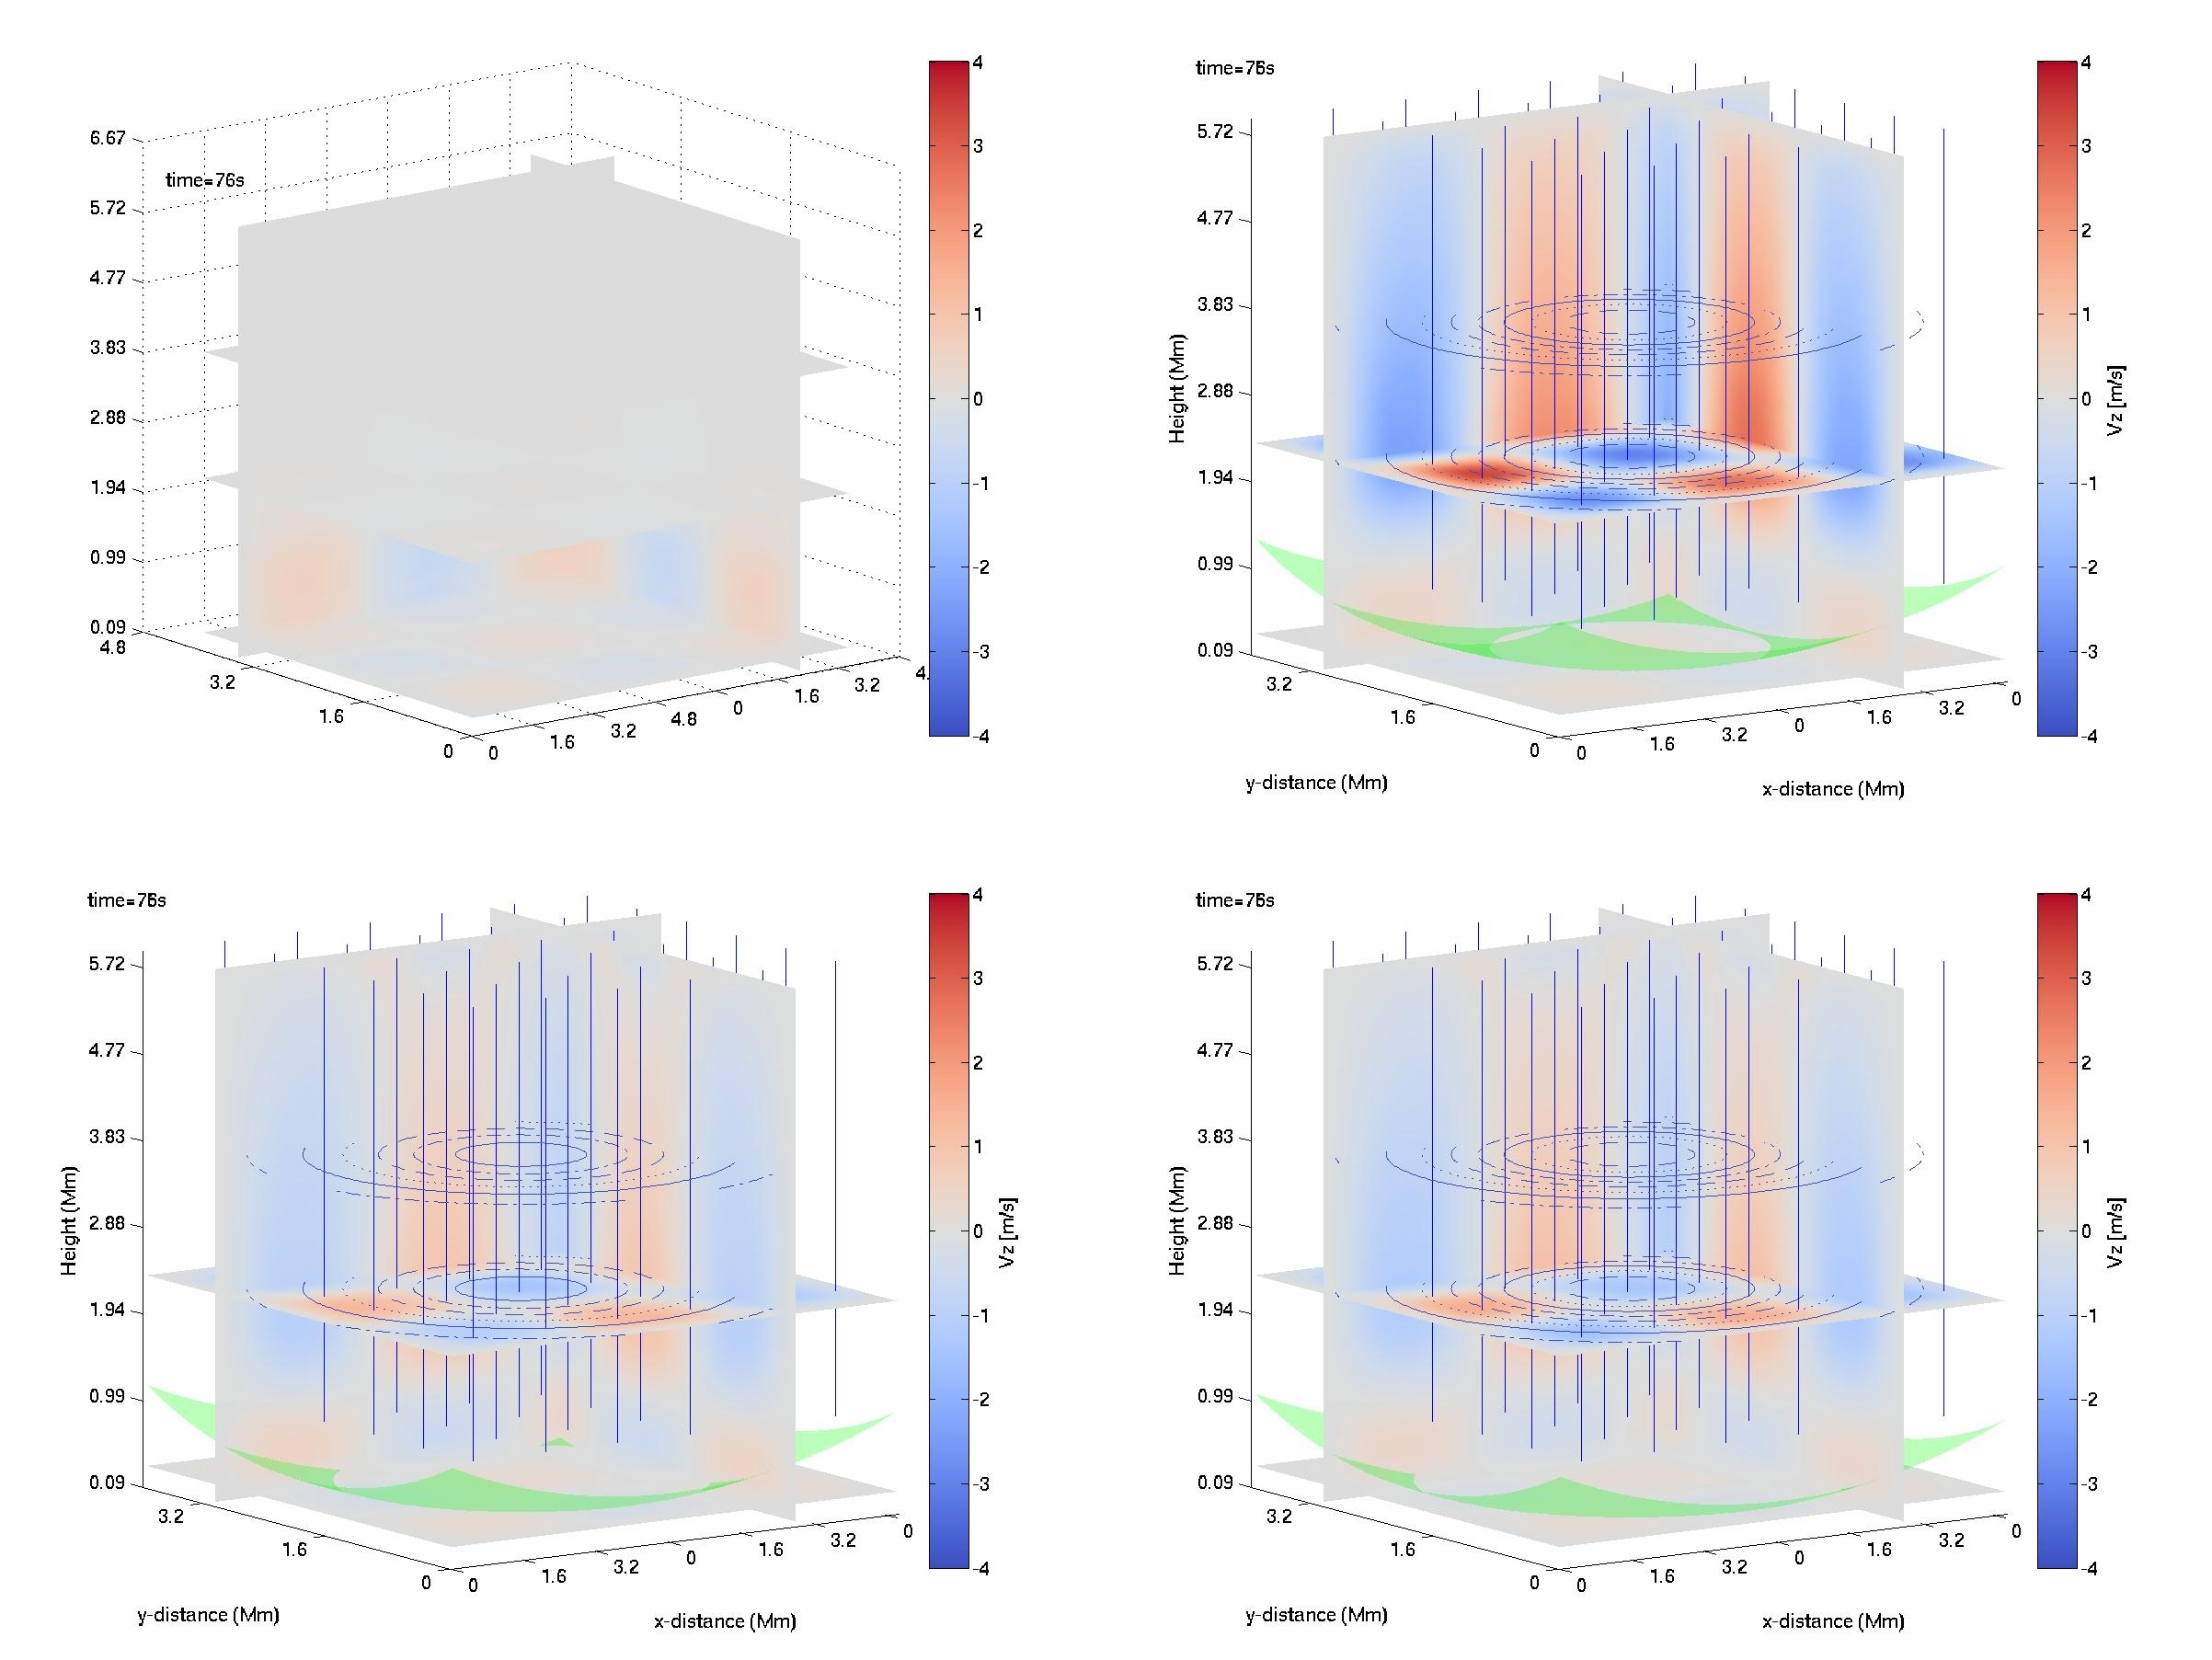
\includegraphics[scale=0.15]{imrescale/vz_0G_50G_75G_100G_76.jpg}
%\caption{Vertical Component of the Velocity for Different Sections of the Simulation for 76s, comparing different strengths for the vertical field magnetic field of 0G, 50G, 75G and 100G}
%\caption{Initial Magnetic Field Configuration, radial field distribution, uniform in the vertical direction with a maximum value of 100G }
%\end{figure}




\begin{figure}
\centering
\label{dt_vvert_100G_300s_180s}
%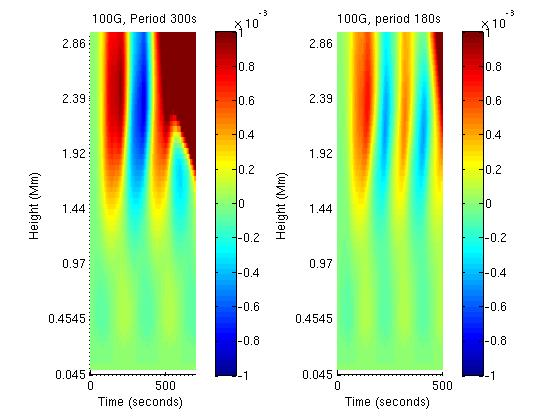
\includegraphics[scale=0.475]{imrescale/dt_vvert_100G_300s_180s.jpg}
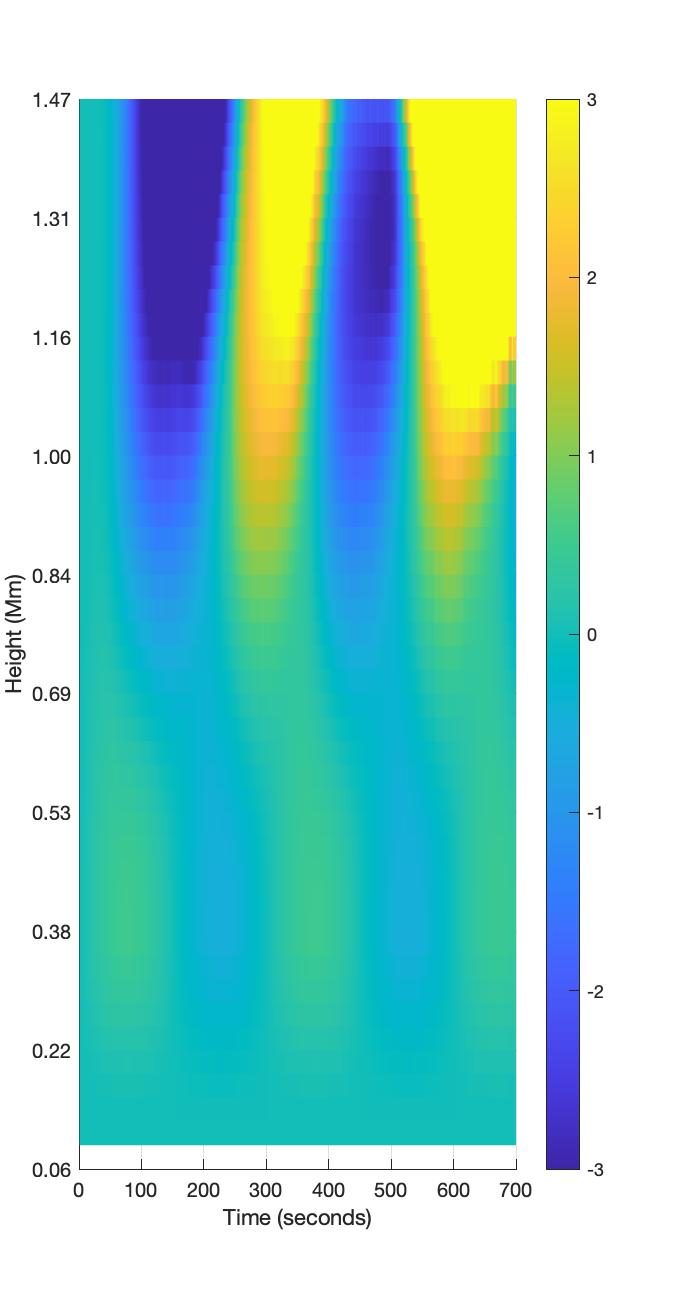
\includegraphics[scale=0.3]{imrescale/dt-5b2_2_100G-midchrom.jpg}
\caption{Distance-time plot of the vertical component of the velocity in the mid chromosphere.}
%\caption{Energy Flux for the mid-section of the Simulation for 76s, 150s, 225s and 330s for a vertical field with maximum field of 50G }
\end{figure}



To determine how the propagation of the wave energy is influenced by the magnetic field strength, we compute the time averaged wave energy flux integrated over the cross-sectional area of the simulation box at different heights. The area of integration is perpendicular to the model $z$-axis.
\begin{equation}
F_{int}= \frac{1}{t_{max}} \int_{0}^{t_{max}} \int {\mathbf F}_{wave} \cdot d{\mathbf A}dt,
\label{e11}
\end{equation}
where the wave energy flux $\bf{F}_{wave}$ is given by
$$
{\mathbf F}_{wave}=\tilde{p}_{k} {\mathbf v}+\tilde{\mathbf B}\cdot {\mathbf B_{b}}{\mathbf v}+{\mathbf v}\cdot \tilde{\mathbf B}{\mathbf B_{b}} .
$$
The expression for the wave energy flux is dependent on the perturbed kinetic pressure, $\tilde{p}_{k}$, given by \citet{Bogdan2003}
$$
\tilde{p}_{k}=\left(\gamma - 1\right)\left( \tilde{e}-\frac{ \left( \tilde{\rho} +\rho_b \right){\mathbf v}^2}{2}-\frac{{\mathbf B}^2}{2}\right).
$$


Using equation (\ref{e11}), we computed the energy flux integral for each of the drivers at different atmospheric heights and averaged over the total time. We compute the ratio of this integrated energy flux to the integrated energy flux at the location of the driver, the resulting values are shown in table \ref{energyflux}.



With the exception of the 75G field case it appears that the energy flux is enhanced for increasing values for the vertical magnetic field. In figure \ref{energyfluxratio_50G_75G_100G_line} we plot the ratio of the integrated energy flux ratio for different values of the field at different heights and for the different vertical field values ( the blue, orange and red  are for field values of 50G, 75G and 100G respectively). This plot demonstrates that for higher B-field magnitudes the energy propagation is suppressed, this is interesting because this is consistent with observations and other simulation results which demonstrate an enhancement for inclined fields.

%%ratios for two sets of simulations. In the first case we show the energy flux ratios for our drivers each delivering the same amount of energy, in the second case (figure 
%\ref{Fig19}
%%), we plot the energy ratios for another set of simulations but where we kept the driver amplitude fixed at the same amplitude for all mode numbers and driver frequencies. The energy flux ratio is the ratio of the energy flux at a given height to the energy flux at the location of the driver. 

\begin{figure}
    \label{energyfluxratio_50G_75G_100G_line}
    \centering
    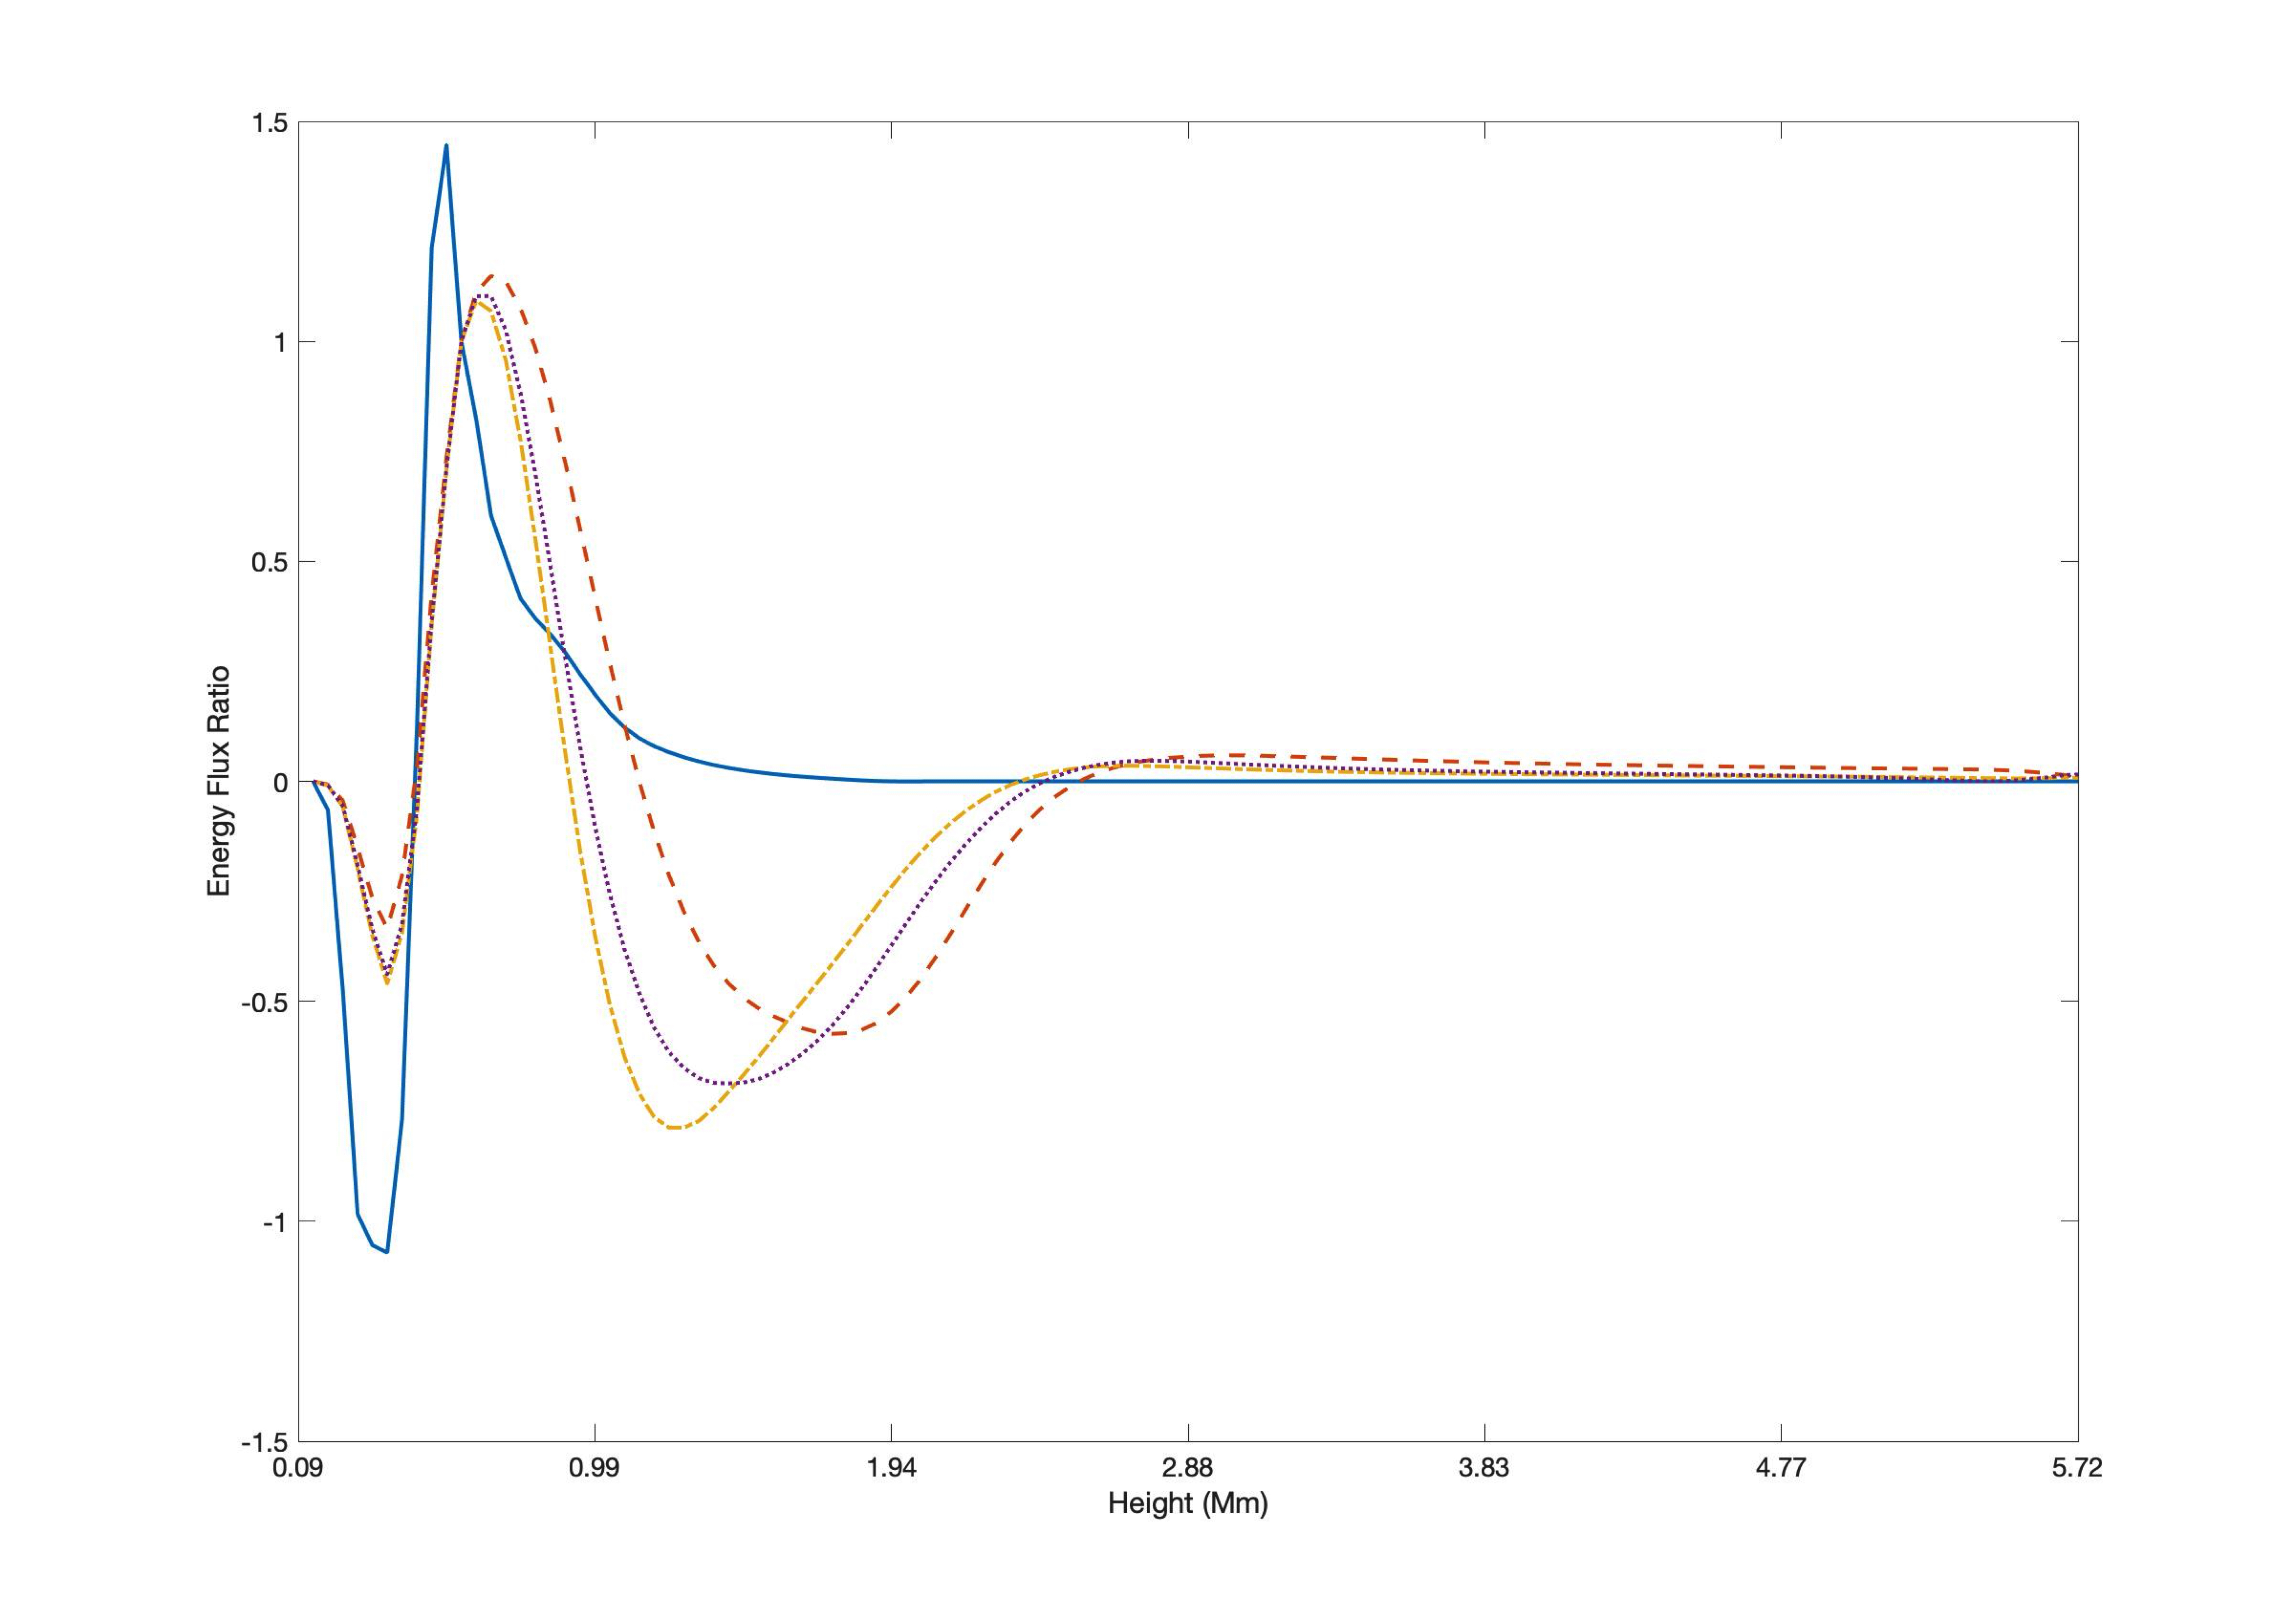
\includegraphics[scale=0.425]{imrescale/energyfluxratio.jpg}
    \caption{Shows the Ratio of the Integrated Energy Flux ratio for different values of the field, Blue 50G, Orange 75G, Red 100GMm}
\end{figure}

\begin{figure}
    \centering
    \label{fft_sim}
    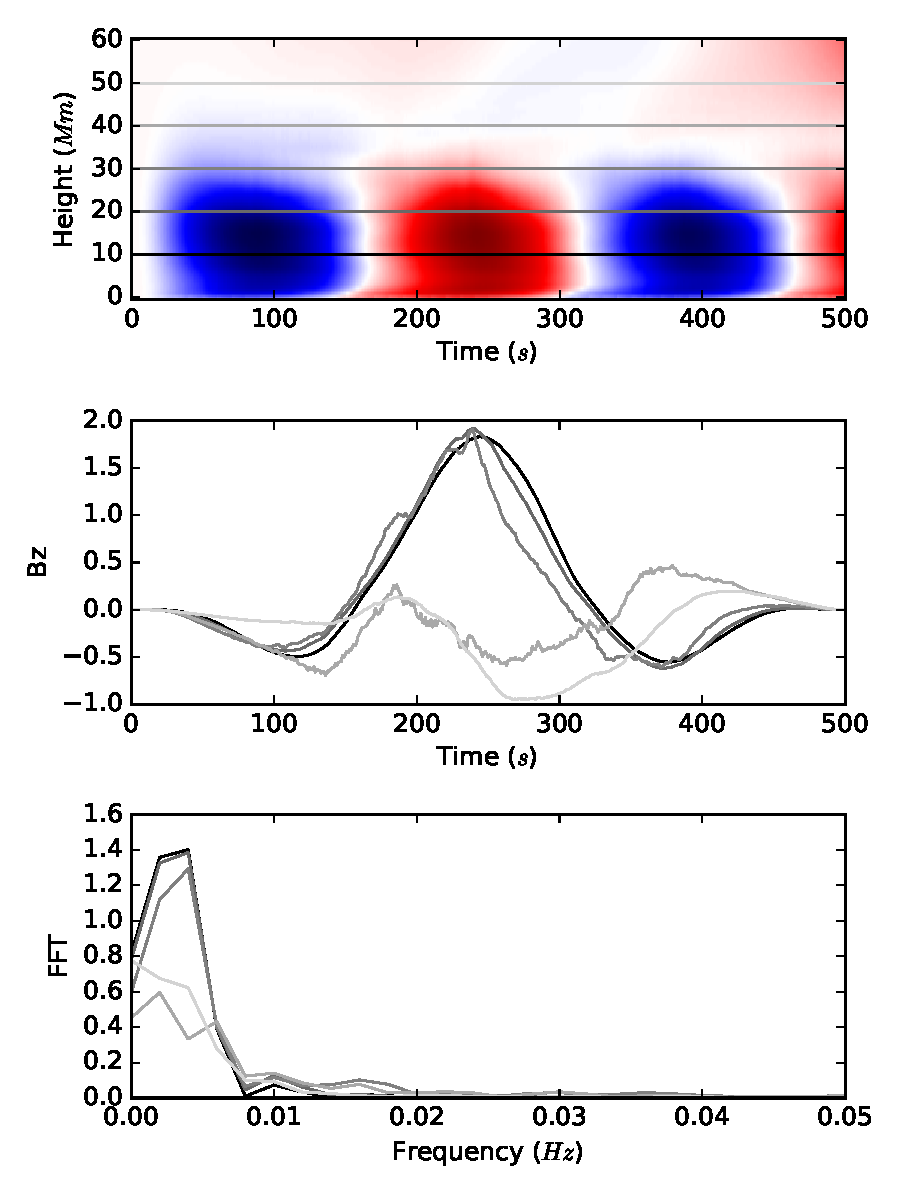
\includegraphics[scale=0.55]{imrescale/fft_sim.pdf}
    \caption{Temporal analysis of $Bz$ vertical slices at $2$ $Mm$. The top panel shows the selected vertical slices, indicated by gray colours. The middle panel demostrates the obtained signal after applying a Hanning window function. The bottom panel shows the result of the FFT analysis based on the $5$ selected vertical $Bz$ slices.}

    \centering
    \label{fft_sim}
    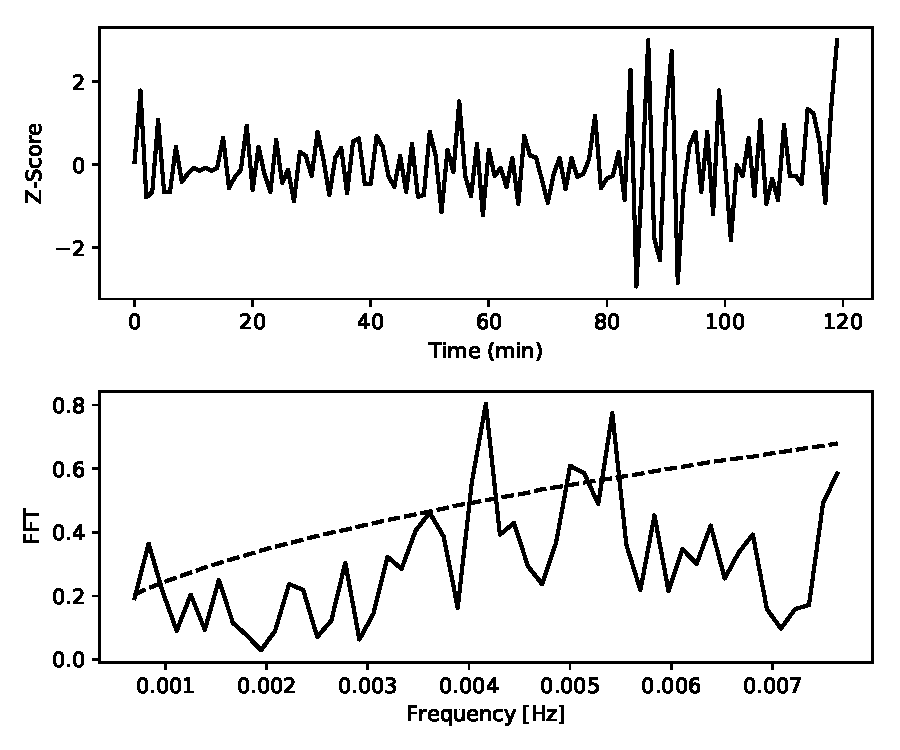
\includegraphics[scale=0.55]{imrescale/fft_obs.pdf}
    \caption{Temporal analysis of pixel intensity based on AIA 1600{\AA} between 18:00 UT to 20:00 UT on 22 August 2010. The upper panel shows the temporal variation of the Z-Score (detrended and normalised pixel intensity data). The lower panel shows the FFT of the analysed observational data. }
\end{figure}

\begin{figure}
    \label{obs}
    \centering
    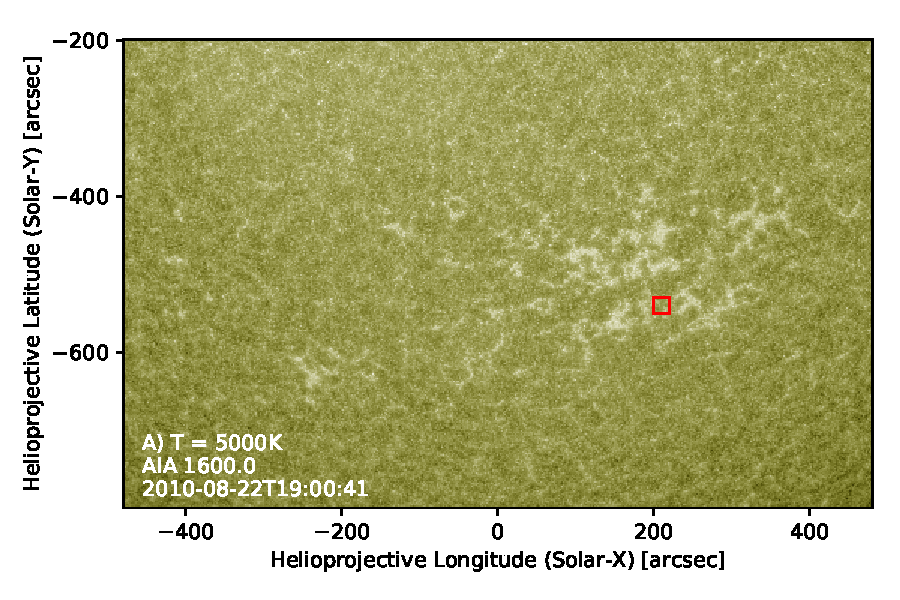
\includegraphics[scale=0.5]{imrescale/obs_data.pdf}
    \caption{The selected pixel from the start of the investigate time series at 18:00 UT on 22 August 2010. The pixel is indicated by red rectangle.}
\end{figure}

\section{Frequency Analysis}

Panel $A$ of Figure \ref{fft_sim} shows a vertical slice of $Bz$ over time based on the simulation with the initial magnetic field configuration with a maximum value of 100 $G$. The vertical axis represents the height in $Mm$ and the horizontal axis is the time dimension, measured in seconds. From this 2-dimensional plain, we selected $5$ layers, indicated by vertical grey lines. Panel $B$ of Figure \ref{fft_sim} displays the temporal variation of the selected layers, indicated by different grey shade colours. The time series do not feature non-stationary behaviour, therefore, further transformations (such as de-trending, smoothing or differentiation) are not needed, Although, Hanning-window function is still applied to avoid leakage effect when performing Fast Fourier Transformation (FFT).  

FFT is applied (Panel $C$) for investigating any oscillatory behaviour in the analysed signal. A significant oscillatory pattern is found with frequency range of $3.75$ - $4$ $mHz$, corresponding a period range of $4.2$ - $4.4$ minutes. FFT was also performed based on other simulations with different initial magnetic field configurations (with a maximum value of 0 $G$, 50 $G$ 75 $G$ and 100 $G$). These investigations all showed similar oscillatory behaviour, therefore, we present one FFT as a representative example. 

Next, temporal analysis for observational data is performed for confirming the obtained oscillatory behaviour. We investigate intensity oscillations in the solar atmosphere observed by SDO/AIA. The passband 1600 {\AA} is selected because our simulation mainly focuses on lower atmospheric regions, i.e. photosphere and chromosphere. The cadence of 1600 {\AA} images is 24 seconds, therefore it is suitable for studying relatively high-frequency oscillations such as the obtained $4$ $mHz$.

The initial magnetic field configuration of our model is a standing magnetic tube, passing through the chromosphere and the lower corona. Therefore, We chose to sample a typical active region. The selected area contains a small sunspot (solar pore), presumably featuring similar magnetic structure as our simulation. From each observation, a single pixel is selected, yielding a $0.35$ $Mm$ by $0.35$ $Mm$ area. The obtained time series shows non-stationary behaviour, therefore, the observed linear trend is removed by taking the first difference $\Delta  y_{t}$ of the data. The first difference is defined as the the difference between consecutive observations $y_{t}$ and $y_{t-1}$. Furthermore, the times series is also normalised by applying standard scores (Z-scores), defined by:

\begin{equation}
	Z_{i} = \frac {T_{i} - \overline{T}}  {\sigma(T)},
	\label{z_score}
\end{equation}

where, the parameter $\overline{T}$ is the mean of the time series and the parameter $\sigma(T)$ is defined as the standard deviation of the data. Panel $A$ of Figure \ref{fft_sim} demonstrates the trend removed and normalised time series. Panel $B$ of Figure \ref{fft_sim} shows the result of the applied FFT technique. The dashed line is the significance level ($3 \sigma$) which is calculated by Monte-Carlo method. The original data showed red noise signature which transformed to blue noise after differentiating the data. We have generated 1 million blue noise signatures $N_{b}$ and calculated the standard deviation $\sigma(N_{b})$ and the mean $\overline{N_{b}}$ of the simulated noise, providing our significance level $S$:

\begin{equation}
    S = \overline{N_{b}} + 3 \sigma(N_{b}).
\end{equation}

A significant period is found with frequency range of $4-4.2$ $mHz$, corresponding a period range of $4$ - $4.2$ minutes, which is close to the period found in simulation data. Another significant peak is found with period around $3$ minutes which may be an indication of another global oscillation.

\section{Conclusion}

In this paper we have presented results for a series of MHD simulations of an extended oscillator at the base of a model solar atmosphere. We have shown that energy is propagated by slow magnetosonic modes. Slow and fast magnetosonic modes are responsible for carrying some energy back to the chromosphere and the photosphere. The results exhibit a small frequency shift  for different values of the magnetic field closer inspection of the energy flux propagation results indicative of enhanced energy flux propagation for inclined magnetic fields. The obtained periodic behaviour is confirmed by observational data, featuring similar frequencies based on the intensity times series of SDO images. The frequency shift measured from the temporal analysis of the observational and simulation data is larger than would be expected from the analysis of \citet{Hindman1996}. 
%ROBERTUS ADD COMMENTS HERE
This can be understood in part by referring to the work of \citet{Campbell1989}.
%ROBERTUS ADD COMMENTS HERE

It is encouraging that the results presented here are consistent with the behaviour exhibited  by earlier work. Future work will address simulation runs over longer time periods and for inclined fields. There is an issue that due to the extended nature of the driver the amplitudes used may be responsible for delivering vast quantities of energy into the solar atmosphere and for driving a highly numerically unstable system and inducing extremely large shocks \citet{Santamaria2015}. 
%e.g. cite reference Solar Physics Fedun et al 2009 oscillatory response 3d solar atmosphere to leakage of photospheric motions

%% If you wish to include an acknowledgments section in your paper,
%% separate it off from the body of the text using the \acknowledgments
%% command.

\section{Acknowledgments}
\acknowledgments

The authors thank P. H. Keys for providing the wavelet tools to analyse the related SDO data M.Korsos for the preparation of Figure 1, the Science and Technology Facilities Council (STFC), UK for the support they received.  RE acknowledges the support received from the the Royal Society (UK). We acknowledge IT Services at The University of Sheffield for the provision of the High Performance Computing Service.


%% To help institutions obtain information on the effectiveness of their 
%% telescopes the AAS Journals has created a group of keywords for telescope 
%% facilities.
%
%% Following the acknowledgments section, use the following syntax and the
%% \facility{} or \facilities{} macros to list the keywords of facilities used 
%% in the research for the paper.  Each keyword is check against the master 
%% list during copy editing.  Individual instruments can be provided in 
%% parentheses, after the keyword, but they are not verified.

%%\vspace{5mm}
%%\facilities{HST(STIS), Swift(XRT and UVOT), AAVSO, CTIO:1.3m,
%%CTIO:1.5m,CXO}

%% Similar to \facility{}, there is the optional \software command to allow 
%% authors a place to specify which programs were used during the creation of 
%% the manusscript. Authors should list each code and include either a
%% citation or url to the code inside ()s when available.

\software{SMAUG \citep{Griffiths2015}, SAC \citep{Shelyag2008},             
          VAC \citep{Toth1996}
          }

%% Appendix material should be preceded with a single \appendix command.
%% There should be a \section command for each appendix. Mark appendix
%% subsections with the same markup you use in the main body of the paper.

%% Each Appendix (indicated with \section) will be lettered A, B, C, etc.
%% The equation counter will reset when it encounters the \appendix
%% command and will number appendix equations (A1), (A2), etc. The
%% Figure and Table counter will not reset.

%%\appendix



%% The reference list follows the main body and any appendices.
%% Use LaTeX's thebibliography environment to mark up your reference list.
%% Note \begin{thebibliography} is followed by an empty set of
%% curly braces.  If you forget this, LaTeX will generate the error
%% "Perhaps a missing \item?".
%%
%% thebibliography produces citations in the text using \bibitem-\cite
%% cross-referencing. Each reference is preceded by a
%% \bibitem command that defines in curly braces the KEY that corresponds
%% to the KEY in the \cite commands (see the first section above).
%% Make sure that you provide a unique KEY for every \bibitem or else the
%% paper will not LaTeX. The square brackets should contain
%% the citation text that LaTeX will insert in
%% place of the \cite commands.

%% We have used macros to produce journal name abbreviations.
%% \aastex provides a number of these for the more frequently-cited journals.
%% See the Author Guide for a list of them.

%% Note that the style of the \bibitem labels (in []) is slightly
%% different from previous examples.  The natbib system solves a host
%% of citation expression problems, but it is necessary to clearly
%% delimit the year from the author name used in the citation.
%% See the natbib documentation for more details and options.

\begin{thebibliography}{}

\bibitem[{{Campbell} and {Roberts} (1989)}]{Campbell1989}
 {Campbell}, W.~R. and {Roberts}, B.\ 1989. {The Influence of a Chromospheric Magnetic Field on the Solar p- and f-Modes} \apj, 338, 538. doi:10.1086/167216

\bibitem[{{Carlsson} and {Stein}(1995)}]{Carlsson1995}
{Carlsson}, M., {Stein}, R.~F., 1995. {Does a nonmagnetic solar chromosphere
  exist?} \apjl 440, L29--L32.

\bibitem[{{Caunt} and {Korpi}(2001)}]{Caunt2001}
{Caunt}, S.~E., {Korpi}, M.~J., Apr. 2001. A {3D} {MHD} model of astrophysical
  flows: Algorithms, tests and parallelisation. \aap 369, 706--728.

\bibitem[{{Fedun} et~al.(2009){Fedun}, {Erd{\'e}lyi}, and
  {Shelyag}}]{Fedun2009}
{Fedun}, V., {Erd{\'e}lyi}, R., {Shelyag}, S., Sep. 2009. {Oscillatory Response
  of the 3D Solar Atmosphere to the Leakage of Photospheric Motion}. \solphys
  258, 219--241.

\bibitem[{{Fedun}, V. and {Shelyag}, S. and {Verth}, G. and {Mathioudakis}, M. and
         {Erd{\'e}lyi}, R.}]{Fedun2011}
{Fedun}, V., {Erd{\'e}lyi}, R., {Shelyag}, S., Sep. 2009. {MHD waves generated by high-frequency photospheric vortex motions}. Annales Geophysicae
  29, 1029-1035.

\bibitem[{{Griffiths} et~al.(2017){Griffiths}, {Erd{\'e}lyi}, and
  {Fedun}}]{Griffiths2017}
{Griffiths}, M., {Erd{\'e}lyi}, R., {Fedun}, V., 2017. {Videos of
  Magnetohydrodynamics Simulations of Solar Atmosphere Wave Dynamics Generated
  by Solar Global Oscillating Eigenmodes}.
\newline \url{https://figshare.com/articles/Videos_of_Magnetohydrodynamics_Simulations_of_Solar_Atmosphere_Wave_Dynamics_Generated_by_Solar_Global_Oscillating_Eigenmodes/4818490}

\bibitem[{{Griffiths} et~al.(2017){Griffiths}, {Erd{\'e}lyi}}]{Griffiths2018}
{Griffiths}, M., {Erd{\'e}lyi}, R., {Fedun}, V., 2018. {Videos of p-Mode Oscillations in Highly Gravitationally Stratified Magnetic Solar Atmospheres}.
\newline \url{https://figshare.com/articles/Videos_of_Magnetohydrodynamics_Simulations_of_Solar_Atmosphere_Wave_Dynamics_Generated_by_Solar_Global_Oscillating_Eigenmodes/4818490}

\bibitem[{{Griffiths} et~al.(2015){Griffiths}, {Fedun}, and
  {Erd{\'e}lyi}}]{Griffiths2015}
{Griffiths}, M.~K., {Fedun}, V., {Erd{\'e}lyi}, R., 2015. {A Fast MHD Code for
  Gravitationally Stratified Media using Graphical Processing Units: SMAUG}.
  Journal of Astrophysics and Astronomy 36, 197--223.


\bibitem[{{Griffiths} et~al.(2018)}]{Griffiths2018}
{Griffiths}, M.~K., {Fedun}, V., {Erd{\'e}lyi}, R., and {Zheng},R.,
{Solar atmosphere wave dynamics generated by solar global oscillating
  eigenmodes}.{Advances in Space Research}, 61: 720--737, January 2018.


\bibitem[{{Hindman} et~al.(1996)}]{Hindman1996}
{Hindman}, B.~W. and {Zweibel}, E.~G. and {Cally}, P.~S., Mar. 1996. {Driven Acoustic Oscillations within a Vertical Magnetic Field}. \apj 459, 760--772.

\bibitem[{{Kalkofen}(2012)}]{Kalkofen2012}
{Kalkofen}, W., 2012. {The Validity of Dynamical Models of the Solar
  Atmosphere}. \solphys 276, 75--95.

\bibitem[{{Khomenko} and {Calvo Santamaria}(2013)}]{Khomenko2013}
{Khomenko}, E., {Calvo Santamaria}, I., 2013. {Magnetohydrodynamic waves driven
  by p-modes}. Journal of Physics Conference Series 440~(1), 012048.

\bibitem[{{Leenaarts} et~al.(2011){Leenaarts}, {Carlsson}, {Hansteen}, and
  {Gudiksen}}]{Leenaarts2011}
{Leenaarts}, J., {Carlsson}, M., {Hansteen}, V., {Gudiksen}, B.~V., 2011. {On
  the minimum temperature of the quiet solar chromosphere}. \aap 530, A124.


\bibitem[{{Leighton}(1960)}]{Leighton1960}
{Leighton}, R.~B., 1960. In: {Thomas}, R.~N. (Ed.), Aerodynamic Phenomena in
  Stellar Atmospheres. Vol.~12 of IAU Symposium. pp. 321--325.

\bibitem[{{Malins}(2007)}]{Malins2007A}
{Malins}, C., 2007. {On transition region convection cells in simulations of
  $\{$p$\}$-mode propagation}. Astronomische Nachrichten 328, 752--755.


\bibitem[{{McWhirter} et~al.(1975){McWhirter}, {Thonemann}, and
  {Wilson}}]{McWhirter1975}
{McWhirter}, R.~W.~P., {Thonemann}, P.~C., {Wilson}, R., 1975. {The heating of
  the solar corona. II - A model based on energy balance}. \aap 40, 63--73.

\bibitem[{{Murawski} and {Zaqarashvili}(2010)}]{Murawski2010}
{Murawski}, K., {Zaqarashvili}, T.~V., 2010. {Numerical simulations of spicule
  formation in the solar atmosphere}. \aap 519, 9.

\bibitem[{{Calvo Santamaria}, {Khomenko} and {Collados}  (2015)}]{Santamaria2015}
 {Calvo Santamaria}, I., {Khomenko}, E.,  and {Collados}, M., 2015. {Magnetohydrodynamic wave propagation from the subphotosphere to the corona in an arcade-shaped magnetic field with a null point}. \aap 577, A70.

\bibitem[{{Shelyag} et~al.(2008){Shelyag}, {Fedun}, and
  {Erd{\'e}lyi}}]{Shelyag2008}
{Shelyag}, S., {Fedun}, V., {Erd{\'e}lyi}, R., 2008. {Magnetohydrodynamic code
  for gravitationally-stratified media}. \aap 486, 655--662.

\bibitem[{{T{\'o}th}(1996)}]{Toth1996}
{T{\'o}th}, G., 1996. {A General Code for Modeling {MHD} Flows on Parallel
  Computers: Versatile Advection Code}. Astrophysical Letters and
  Communications 34, 245.

\bibitem[{{Vernazza} et~al.(1981){Vernazza}, {Avrett}, and
  {Loeser}}]{Vernazza1981}
{Vernazza}, J.~E., {Avrett}, E.~H., {Loeser}, R., 1981. {Structure of the solar
  chromosphere. III - Models of the EUV brightness components of the
  quiet-sun}. Astrophysical Journal Supplement Series 45, 635--725.

\bibitem[{{Vigeesh} et~al.(2012)    {Vigeesh}, {Fedun},{Hasan} and {Erd{\'e}lyi}}]{Vigeesh2012}
{Vigeesh}, G.,{Fedun}, V.,{Hasan}, S.~S., {Erd{\'e}lyi}, R.,  Jan. 2012. {Three-dimensional Simulations of Magnetohydrodynamic Waves in Magnetized Solar Atmosphere}. \apj
  755, 1--18.

\bibitem[{Kontogiannis} et~al.(2010){Kontogiannis}, {Tsiropoula}, and
  {Tziotziou}]{Kontogiannis2010}
I.~{Kontogiannis}, G.~{Tsiropoula}, and K.~{Tziotziou}.
\newblock {Power halo and magnetic shadow in a solar quiet region observed in
  the H{$\alpha$} line}.
\newblock \emph{\aap}, 510:\penalty0 A41, February 2010.
\newblock \doi{10.1051/0004-6361/200912841}.

\bibitem[{V{\"o}gler} et~al.(2005){V{\"o}gler}, {Shelyag}, {Sch{\"u}ssler},
  {Cattaneo}, {Emonet}, and {Linde}]{Vogler2005}
A.~{V{\"o}gler}, S.~{Shelyag}, M.~{Sch{\"u}ssler}, F.~{Cattaneo}, T.~{Emonet},
  and T.~{Linde}.
\newblock {Simulations of magneto-convection in the solar photosphere.
  Equations, methods, and results of the MURaM code}.
\newblock \emph{\aap}, 429:\penalty0 335--351, January 2005.
\newblock \doi{10.1051/0004-6361:20041507}.

\bibitem[{Gudiksen} et~al.(2011){Gudiksen}, {Carlsson}, {Hansteen}, {Hayek},
  {Leenaarts}, and {Mart{\'{\i}}nez-Sykora}]{Gudiksen2011}
B.~V. {Gudiksen}, M.~{Carlsson}, V.~H. {Hansteen}, W.~{Hayek}, J.~{Leenaarts},
  and J.~{Mart{\'{\i}}nez-Sykora}.
\newblock {The stellar atmosphere simulation code Bifrost. Code description and
  validation}.
\newblock \emph{\aap}, 531:\penalty0 A154, July 2011.
\newblock \doi{10.1051/0004-6361/201116520}.

\bibitem[{{Bogdan} et~al.(2003){Bogdan}, {Carlsson}, {Hansteen}, {McMurry},
  {Rosenthal}, {Johnson}, {Petty-Powell}, {Zita}, {Stein}, {McIntosh}, and
  {Nordlund}}]{Bogdan2003}
{Bogdan}, T.~J., {Carlsson}, M., {Hansteen}, V.~H., {McMurry}, A., {Rosenthal},
  C.~S., {Johnson}, M., {Petty-Powell}, S., {Zita}, E.~J., {Stein}, R.~F.,
  {McIntosh}, S.~W., {Nordlund}, {\AA}., 2003. {Waves in the Magnetized Solar
  Atmosphere. II. Waves from Localized Sources in Magnetic Flux
  Concentrations}. \apj 599, 626--660.



%%\bibitem[Astropy Collaboration et al.(2013)]{2013A&A...558A..33A} Astropy Collaboration, Robitaille, T.~P., Tollerud, E.~J., et al.\ 2013, \aap, 558, A33 
%%\bibitem[Bertin \& Arnouts(1996)]{1996A&AS..117..393B} Bertin, E., \& Arnouts, S.\ 1996, \aaps, 117, 393 
%%\bibitem[Corrales(2015)]{2015ApJ...805...23C} Corrales, L.\ 2015, \apj, 805, 23
%%\bibitem[Ferland et al.(2013)]{2013RMxAA..49..137F} Ferland, G.~J., Porter, R.~L., van Hoof, P.~A.~M., et al.\ 2013, \rmxaa, 49, 137
%%\bibitem[Hanisch \& Biemesderfer(1989)]{1989BAAS...21..780H} Hanisch, R.~J., \& Biemesderfer, C.~D.\ 1989, \baas, 21, 780 
%%\bibitem[Lamport(1994)]{lamport94} Lamport, L. 1994, LaTeX: A Document Preparation System, 2nd Edition (Boston, Addison-Wesley Professional)
%%\bibitem[Schwarz et al.(2011)]{2011ApJS..197...31S} Schwarz, G.~J., Ness, J.-U., Osborne, J.~P., et al.\ 2011, \apjs, 197, 31  
%%\bibitem[Vogt et al.(2014)]{2014ApJ...793..127V} Vogt, F.~P.~A., Dopita, M.~A., Kewley, L.~J., et al.\ 2014, \apj, 793, 127  

\end{thebibliography}

%% This command is needed to show the entire author+affilation list when
%% the collaboration and author truncation commands are used.  It has to
%% go at the end of the manuscript.
%\allauthors

%% Include this line if you are using the \added, \replaced, \deleted
%% commands to see a summary list of all changes at the end of the article.
%\listofchanges

\end{document}

% End of file `sample62.tex'.
